\documentclass[twoside]{book}

% Packages required by doxygen
\usepackage{fixltx2e}
\usepackage{calc}
\usepackage{doxygen}
\usepackage[export]{adjustbox} % also loads graphicx
\usepackage{graphicx}
\usepackage[utf8]{inputenc}
\usepackage{makeidx}
\usepackage{multicol}
\usepackage{multirow}
\PassOptionsToPackage{warn}{textcomp}
\usepackage{textcomp}
\usepackage[nointegrals]{wasysym}
\usepackage[table]{xcolor}

% NLS support packages
\usepackage[french]{babel}

% Font selection
\usepackage[T1]{fontenc}
\usepackage[scaled=.90]{helvet}
\usepackage{courier}
\usepackage{amssymb}
\usepackage{sectsty}
\renewcommand{\familydefault}{\sfdefault}
\allsectionsfont{%
  \fontseries{bc}\selectfont%
  \color{darkgray}%
}
\renewcommand{\DoxyLabelFont}{%
  \fontseries{bc}\selectfont%
  \color{darkgray}%
}
\newcommand{\+}{\discretionary{\mbox{\scriptsize$\hookleftarrow$}}{}{}}

% Page & text layout
\usepackage{geometry}
\geometry{%
  a4paper,%
  top=2.5cm,%
  bottom=2.5cm,%
  left=2.5cm,%
  right=2.5cm%
}
\tolerance=750
\hfuzz=15pt
\hbadness=750
\setlength{\emergencystretch}{15pt}
\setlength{\parindent}{0cm}
\setlength{\parskip}{3ex plus 2ex minus 2ex}
\makeatletter
\renewcommand{\paragraph}{%
  \@startsection{paragraph}{4}{0ex}{-1.0ex}{1.0ex}{%
    \normalfont\normalsize\bfseries\SS@parafont%
  }%
}
\renewcommand{\subparagraph}{%
  \@startsection{subparagraph}{5}{0ex}{-1.0ex}{1.0ex}{%
    \normalfont\normalsize\bfseries\SS@subparafont%
  }%
}
\makeatother

% Headers & footers
\usepackage{fancyhdr}
\pagestyle{fancyplain}
\fancyhead[LE]{\fancyplain{}{\bfseries\thepage}}
\fancyhead[CE]{\fancyplain{}{}}
\fancyhead[RE]{\fancyplain{}{\bfseries\leftmark}}
\fancyhead[LO]{\fancyplain{}{\bfseries\rightmark}}
\fancyhead[CO]{\fancyplain{}{}}
\fancyhead[RO]{\fancyplain{}{\bfseries\thepage}}
\fancyfoot[LE]{\fancyplain{}{}}
\fancyfoot[CE]{\fancyplain{}{}}
\fancyfoot[RE]{\fancyplain{}{\bfseries\scriptsize Généré par Doxygen }}
\fancyfoot[LO]{\fancyplain{}{\bfseries\scriptsize Généré par Doxygen }}
\fancyfoot[CO]{\fancyplain{}{}}
\fancyfoot[RO]{\fancyplain{}{}}
\renewcommand{\footrulewidth}{0.4pt}
\renewcommand{\chaptermark}[1]{%
  \markboth{#1}{}%
}
\renewcommand{\sectionmark}[1]{%
  \markright{\thesection\ #1}%
}

% Indices & bibliography
\usepackage{natbib}
\usepackage[titles]{tocloft}
\setcounter{tocdepth}{3}
\setcounter{secnumdepth}{5}
\makeindex

% Hyperlinks (required, but should be loaded last)
\usepackage{ifpdf}
\ifpdf
  \usepackage[pdftex,pagebackref=true]{hyperref}
\else
  \usepackage[ps2pdf,pagebackref=true]{hyperref}
\fi
\hypersetup{%
  colorlinks=true,%
  linkcolor=blue,%
  citecolor=blue,%
  unicode%
}

% Custom commands
\newcommand{\clearemptydoublepage}{%
  \newpage{\pagestyle{empty}\cleardoublepage}%
}

\usepackage{caption}
\captionsetup{labelsep=space,justification=centering,font={bf},singlelinecheck=off,skip=4pt,position=top}

%===== C O N T E N T S =====

\begin{document}

% Titlepage & ToC
\hypersetup{pageanchor=false,
             bookmarksnumbered=true,
             pdfencoding=unicode
            }
\pagenumbering{roman}
\begin{titlepage}
\vspace*{7cm}
\begin{center}%
{\Large C A\+I\+R-\/1 \\[1ex]\large 0.\+1.\+0 }\\
\vspace*{1cm}
{\large Généré par Doxygen 1.8.11}\\
\end{center}
\end{titlepage}
\clearemptydoublepage
\tableofcontents
\clearemptydoublepage
\pagenumbering{arabic}
\hypersetup{pageanchor=true}

%--- Begin generated contents ---
\chapter{Index des structures de données}
\section{Structures de données}
Liste des structures de données avec une brève description \+:\begin{DoxyCompactList}
\item\contentsline{section}{\hyperlink{structcarte}{carte} \\*Définit une carte }{\pageref{structcarte}}{}
\item\contentsline{section}{\hyperlink{structcarte__cell}{carte\+\_\+cell} \\*Définit une cellule d\textquotesingle{}une liste chaînée de cartes }{\pageref{structcarte__cell}}{}
\item\contentsline{section}{\hyperlink{structcarte__liste}{carte\+\_\+liste} \\*Définit une liste chaînée de cartes }{\pageref{structcarte__liste}}{}
\item\contentsline{section}{\hyperlink{structcarte__prop}{carte\+\_\+prop} \\*Définit une propriété d\textquotesingle{}une carte }{\pageref{structcarte__prop}}{}
\end{DoxyCompactList}

\chapter{Index des fichiers}
\section{Liste des fichiers}
Liste de tous les fichiers documentés avec une brève description \+:\begin{DoxyCompactList}
\item\contentsline{section}{src/\hyperlink{bdd_8c}{bdd.\+c} \\*Fonctions de base de données }{\pageref{bdd_8c}}{}
\item\contentsline{section}{src/\hyperlink{bdd_8h}{bdd.\+h} \\*Définitions des fonctions de la base de données }{\pageref{bdd_8h}}{}
\item\contentsline{section}{src/\hyperlink{carte_8c}{carte.\+c} \\*Fonctions de manipulation de l\textquotesingle{}entité \char`\"{}carte\char`\"{} }{\pageref{carte_8c}}{}
\item\contentsline{section}{src/\hyperlink{carte_8h}{carte.\+h} \\*Définition des fonctions et types de cartes }{\pageref{carte_8h}}{}
\end{DoxyCompactList}

\chapter{Documentation des structures de données}
\hypertarget{structcarte}{}\section{Référence de la structure carte}
\label{structcarte}\index{carte@{carte}}


{\ttfamily \#include $<$carte.\+h$>$}



Graphe de collaboration de carte\+:\nopagebreak
\begin{figure}[H]
\begin{center}
\leavevmode
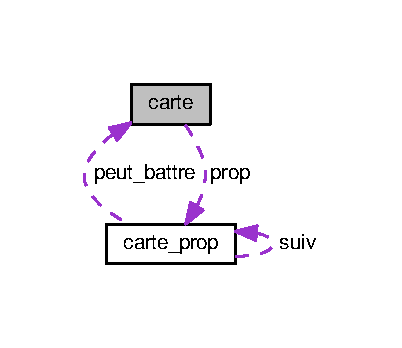
\includegraphics[width=193pt]{structcarte__coll__graph}
\end{center}
\end{figure}
\subsection*{Champs de données}
\begin{DoxyCompactItemize}
\item 
struct \hyperlink{structcarte__prop}{carte\+\_\+prop} $\ast$ {\bfseries prop}\hypertarget{structcarte_aa60e889514f9a3a4d33cc74fe0ad2eff}{}\label{structcarte_aa60e889514f9a3a4d33cc74fe0ad2eff}

\end{DoxyCompactItemize}


\subsection{Description détaillée}
La carte à proprement parler 

La documentation de cette structure a été générée à partir du fichier suivant \+:\begin{DoxyCompactItemize}
\item 
src/\hyperlink{carte_8h}{carte.\+h}\end{DoxyCompactItemize}

\hypertarget{structcarte__cell}{}\section{Référence de la structure carte\+\_\+cell}
\label{structcarte__cell}\index{carte\+\_\+cell@{carte\+\_\+cell}}


Définit une cellule d\textquotesingle{}une liste chaînée de cartes.  




{\ttfamily \#include $<$bdd.\+h$>$}



Graphe de collaboration de carte\+\_\+cell\+:\nopagebreak
\begin{figure}[H]
\begin{center}
\leavevmode
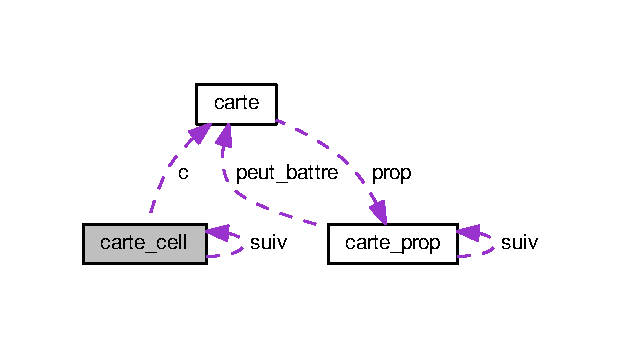
\includegraphics[width=300pt]{structcarte__cell__coll__graph}
\end{center}
\end{figure}
\subsection*{Champs de données}
\begin{DoxyCompactItemize}
\item 
\hyperlink{structcarte}{carte} $\ast$ \hyperlink{structcarte__cell_a2c4496b232d881213e41fe630c3843bb}{c}
\item 
struct \hyperlink{structcarte__cell}{carte\+\_\+cell} $\ast$ \hyperlink{structcarte__cell_aa9b3e04e481fb482711d5d66e4e45924}{suiv}
\end{DoxyCompactItemize}


\subsection{Description détaillée}
Définit une cellule d\textquotesingle{}une liste chaînée de cartes. 

\subsection{Documentation des champs}
\index{carte\+\_\+cell@{carte\+\_\+cell}!c@{c}}
\index{c@{c}!carte\+\_\+cell@{carte\+\_\+cell}}
\subsubsection[{\texorpdfstring{c}{c}}]{\setlength{\rightskip}{0pt plus 5cm}{\bf carte}$\ast$ carte\+\_\+cell\+::c}\hypertarget{structcarte__cell_a2c4496b232d881213e41fe630c3843bb}{}\label{structcarte__cell_a2c4496b232d881213e41fe630c3843bb}
La carte à référencer \index{carte\+\_\+cell@{carte\+\_\+cell}!suiv@{suiv}}
\index{suiv@{suiv}!carte\+\_\+cell@{carte\+\_\+cell}}
\subsubsection[{\texorpdfstring{suiv}{suiv}}]{\setlength{\rightskip}{0pt plus 5cm}struct {\bf carte\+\_\+cell}$\ast$ carte\+\_\+cell\+::suiv}\hypertarget{structcarte__cell_aa9b3e04e481fb482711d5d66e4e45924}{}\label{structcarte__cell_aa9b3e04e481fb482711d5d66e4e45924}
La cellule suivante 

La documentation de cette structure a été générée à partir du fichier suivant \+:\begin{DoxyCompactItemize}
\item 
src/\hyperlink{bdd_8h}{bdd.\+h}\end{DoxyCompactItemize}

\hypertarget{structcarte__liste}{}\section{Référence de la structure carte\+\_\+liste}
\label{structcarte__liste}\index{carte\+\_\+liste@{carte\+\_\+liste}}


Définit une liste chaînée de cartes.  




{\ttfamily \#include $<$bdd.\+h$>$}



Graphe de collaboration de carte\+\_\+liste\+:
\nopagebreak
\begin{figure}[H]
\begin{center}
\leavevmode
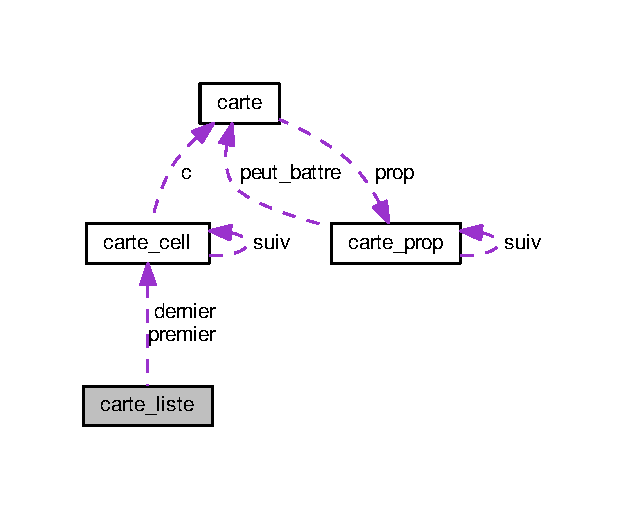
\includegraphics[width=301pt]{structcarte__liste__coll__graph}
\end{center}
\end{figure}
\subsection*{Champs de données}
\begin{DoxyCompactItemize}
\item 
\hyperlink{structcarte__cell}{carte\+\_\+cell} $\ast$ \hyperlink{structcarte__liste_aab2e8cf4d231e6f335d4dc99343d1421}{premier}
\item 
\hyperlink{structcarte__cell}{carte\+\_\+cell} $\ast$ \hyperlink{structcarte__liste_abeffe6f9b0cfe0111b785b92ac2af410}{dernier}
\end{DoxyCompactItemize}


\subsection{Description détaillée}
Définit une liste chaînée de cartes. 

\subsection{Documentation des champs}
\index{carte\+\_\+liste@{carte\+\_\+liste}!dernier@{dernier}}
\index{dernier@{dernier}!carte\+\_\+liste@{carte\+\_\+liste}}
\subsubsection[{\texorpdfstring{dernier}{dernier}}]{\setlength{\rightskip}{0pt plus 5cm}{\bf carte\+\_\+cell}$\ast$ carte\+\_\+liste\+::dernier}\hypertarget{structcarte__liste_abeffe6f9b0cfe0111b785b92ac2af410}{}\label{structcarte__liste_abeffe6f9b0cfe0111b785b92ac2af410}
Le dernier élément de la liste \index{carte\+\_\+liste@{carte\+\_\+liste}!premier@{premier}}
\index{premier@{premier}!carte\+\_\+liste@{carte\+\_\+liste}}
\subsubsection[{\texorpdfstring{premier}{premier}}]{\setlength{\rightskip}{0pt plus 5cm}{\bf carte\+\_\+cell}$\ast$ carte\+\_\+liste\+::premier}\hypertarget{structcarte__liste_aab2e8cf4d231e6f335d4dc99343d1421}{}\label{structcarte__liste_aab2e8cf4d231e6f335d4dc99343d1421}
Le premier élément de la liste 

La documentation de cette structure a été générée à partir du fichier suivant \+:\begin{DoxyCompactItemize}
\item 
src/\hyperlink{bdd_8h}{bdd.\+h}\end{DoxyCompactItemize}

\hypertarget{structcarte__prop}{}\section{Référence de la structure carte\+\_\+prop}
\label{structcarte__prop}\index{carte\+\_\+prop@{carte\+\_\+prop}}


Définit une propriété d\textquotesingle{}une carte.  




{\ttfamily \#include $<$carte.\+h$>$}



Graphe de collaboration de carte\+\_\+prop\+:
\nopagebreak
\begin{figure}[H]
\begin{center}
\leavevmode
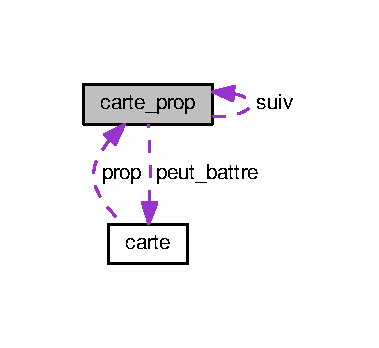
\includegraphics[width=182pt]{structcarte__prop__coll__graph}
\end{center}
\end{figure}
\subsection*{Champs de données}
\begin{DoxyCompactItemize}
\item 
\begin{tabbing}
xx\=xx\=xx\=xx\=xx\=xx\=xx\=xx\=xx\=\kill
union \{\\
\>enum \hyperlink{carte_8h_a2b6a5add5e3db9028dff54f9c1acdde7}{carte\_enseigne} \hyperlink{structcarte__prop_aa01631e22730e71acdae17bec74fcdd3}{enseigne}\\
\>enum \hyperlink{carte_8h_a323916cdb68cd0d5d8a1660ffb45ea4e}{carte\_valeur} \hyperlink{structcarte__prop_a8069caea55ffab4bbdbb27b9d2b1c651}{valeur}\\
\>\hyperlink{structcarte}{carte} $\ast$ \hyperlink{structcarte__prop_a23cb7c2805cd6c447786465937cb0255}{peut\_battre}\\
\} {\bfseries val}\hypertarget{structcarte__prop_a36e90757d299ff149c6884f54e18e84b}{}\label{structcarte__prop_a36e90757d299ff149c6884f54e18e84b}
\\

\end{tabbing}\item 
enum \hyperlink{carte_8h_a71a2818c25230a5e1a239f28c1e6deba}{carte\+\_\+prop\+\_\+type} \hyperlink{structcarte__prop_a434a5fe3ac234b8886126c4ea9acf243}{type}
\item 
struct \hyperlink{structcarte__prop}{carte\+\_\+prop} $\ast$ \hyperlink{structcarte__prop_a0cb42544111674aa11728c2b7392a661}{suiv}
\end{DoxyCompactItemize}


\subsection{Description détaillée}
Définit une propriété d\textquotesingle{}une carte. 

\subsection{Documentation des champs}
\index{carte\+\_\+prop@{carte\+\_\+prop}!enseigne@{enseigne}}
\index{enseigne@{enseigne}!carte\+\_\+prop@{carte\+\_\+prop}}
\subsubsection[{\texorpdfstring{enseigne}{enseigne}}]{\setlength{\rightskip}{0pt plus 5cm}enum {\bf carte\+\_\+enseigne} carte\+\_\+prop\+::enseigne}\hypertarget{structcarte__prop_aa01631e22730e71acdae17bec74fcdd3}{}\label{structcarte__prop_aa01631e22730e71acdae17bec74fcdd3}
Enseigne d\textquotesingle{}une carte (pique, carreaux ...) \index{carte\+\_\+prop@{carte\+\_\+prop}!peut\+\_\+battre@{peut\+\_\+battre}}
\index{peut\+\_\+battre@{peut\+\_\+battre}!carte\+\_\+prop@{carte\+\_\+prop}}
\subsubsection[{\texorpdfstring{peut\+\_\+battre}{peut_battre}}]{\setlength{\rightskip}{0pt plus 5cm}{\bf carte}$\ast$ carte\+\_\+prop\+::peut\+\_\+battre}\hypertarget{structcarte__prop_a23cb7c2805cd6c447786465937cb0255}{}\label{structcarte__prop_a23cb7c2805cd6c447786465937cb0255}
Pointeur vers une carte que la carte courante peut battre \index{carte\+\_\+prop@{carte\+\_\+prop}!suiv@{suiv}}
\index{suiv@{suiv}!carte\+\_\+prop@{carte\+\_\+prop}}
\subsubsection[{\texorpdfstring{suiv}{suiv}}]{\setlength{\rightskip}{0pt plus 5cm}struct {\bf carte\+\_\+prop}$\ast$ carte\+\_\+prop\+::suiv}\hypertarget{structcarte__prop_a0cb42544111674aa11728c2b7392a661}{}\label{structcarte__prop_a0cb42544111674aa11728c2b7392a661}
Pointeur vers la propriété suivante \index{carte\+\_\+prop@{carte\+\_\+prop}!type@{type}}
\index{type@{type}!carte\+\_\+prop@{carte\+\_\+prop}}
\subsubsection[{\texorpdfstring{type}{type}}]{\setlength{\rightskip}{0pt plus 5cm}enum {\bf carte\+\_\+prop\+\_\+type} carte\+\_\+prop\+::type}\hypertarget{structcarte__prop_a434a5fe3ac234b8886126c4ea9acf243}{}\label{structcarte__prop_a434a5fe3ac234b8886126c4ea9acf243}
Champ discriminant pour savoir quel champ de l\textquotesingle{}union lire \index{carte\+\_\+prop@{carte\+\_\+prop}!valeur@{valeur}}
\index{valeur@{valeur}!carte\+\_\+prop@{carte\+\_\+prop}}
\subsubsection[{\texorpdfstring{valeur}{valeur}}]{\setlength{\rightskip}{0pt plus 5cm}enum {\bf carte\+\_\+valeur} carte\+\_\+prop\+::valeur}\hypertarget{structcarte__prop_a8069caea55ffab4bbdbb27b9d2b1c651}{}\label{structcarte__prop_a8069caea55ffab4bbdbb27b9d2b1c651}
Valeur (2, 3, as, roi ...) 

La documentation de cette structure a été générée à partir du fichier suivant \+:\begin{DoxyCompactItemize}
\item 
src/\hyperlink{carte_8h}{carte.\+h}\end{DoxyCompactItemize}

\chapter{Documentation des fichiers}
\hypertarget{bdd_8c}{}\section{Référence du fichier src/bdd.c}
\label{bdd_8c}\index{src/bdd.\+c@{src/bdd.\+c}}


Fonctions de base de données.  


{\ttfamily \#include \char`\"{}bdd.\+h\char`\"{}}\\*
{\ttfamily \#include \char`\"{}carte.\+h\char`\"{}}\\*
{\ttfamily \#include $<$stdlib.\+h$>$}\\*
{\ttfamily \#include $<$stdio.\+h$>$}\\*
{\ttfamily \#include $<$errno.\+h$>$}\\*
Graphe des dépendances par inclusion de bdd.\+c\+:\nopagebreak
\begin{figure}[H]
\begin{center}
\leavevmode
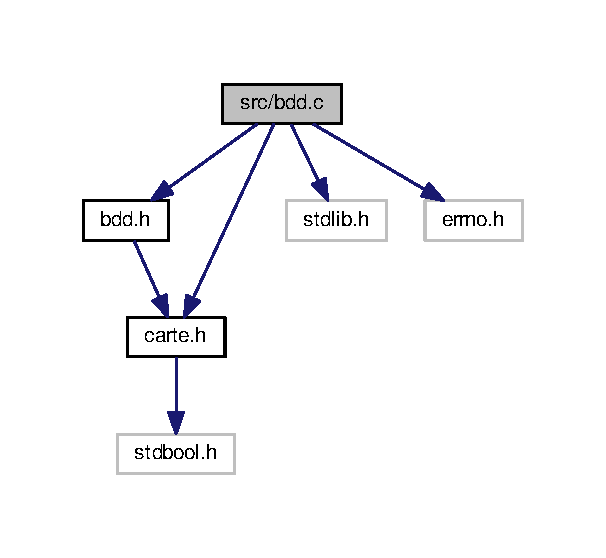
\includegraphics[width=350pt]{bdd_8c__incl}
\end{center}
\end{figure}
\subsection*{Fonctions}
\begin{DoxyCompactItemize}
\item 
\hyperlink{structcarte__cell}{carte\+\_\+cell} $\ast$ \hyperlink{bdd_8c_a87addd1ecffd0863b17cb28d93b9eeac}{air\+\_\+bdd\+\_\+cell\+\_\+creer} (\hyperlink{structcarte}{carte} $\ast$c)
\begin{DoxyCompactList}\small\item\em Alloue et initialise une cellule. \end{DoxyCompactList}\item 
int \hyperlink{bdd_8c_a0042562c59847df384309d7f5ba2068d}{air\+\_\+bdd\+\_\+cell\+\_\+init} (\hyperlink{structcarte__cell}{carte\+\_\+cell} $\ast$cell, \hyperlink{structcarte}{carte} $\ast$c)
\begin{DoxyCompactList}\small\item\em Initialise une cellule. \end{DoxyCompactList}\item 
\hyperlink{structcarte__liste}{carte\+\_\+liste} $\ast$ \hyperlink{bdd_8c_a05d3472e6bc6fa13e2eb6a85e283a34a}{air\+\_\+bdd\+\_\+liste\+\_\+creer} ()
\begin{DoxyCompactList}\small\item\em Alloue et initialise une liste de cellules. \end{DoxyCompactList}\item 
int \hyperlink{bdd_8c_af35c055376980fd980cbc3e92df6cd7e}{air\+\_\+bdd\+\_\+liste\+\_\+init} (\hyperlink{structcarte__liste}{carte\+\_\+liste} $\ast$l)
\begin{DoxyCompactList}\small\item\em Initialise une liste de cellules. \end{DoxyCompactList}\item 
void \hyperlink{bdd_8c_a712e2dd20d20cc921237b8170af2fe52}{air\+\_\+bdd\+\_\+liste\+\_\+free} (\hyperlink{structcarte__liste}{carte\+\_\+liste} $\ast$l)
\begin{DoxyCompactList}\small\item\em Libère de la mémoire une liste de cellules. \end{DoxyCompactList}\item 
int \hyperlink{bdd_8c_a5fc0f20d939cef77b20fe0289cc28af3}{air\+\_\+bdd\+\_\+liste\+\_\+ajouter} (\hyperlink{structcarte__liste}{carte\+\_\+liste} $\ast$l, \hyperlink{structcarte}{carte} $\ast$c)
\begin{DoxyCompactList}\small\item\em Ajoute une carte à la liste. \end{DoxyCompactList}\item 
int \hyperlink{bdd_8c_adf6378260ec8d764e642fc89f7865f5f}{air\+\_\+bdd\+\_\+liste\+\_\+retirer} (\hyperlink{structcarte__liste}{carte\+\_\+liste} $\ast$l, \hyperlink{structcarte}{carte} $\ast$c)
\begin{DoxyCompactList}\small\item\em Reture une carte de la liste. \end{DoxyCompactList}\item 
int \hyperlink{bdd_8c_ab8e2391c7ec0afde492fc38ae88921fd}{air\+\_\+bdd\+\_\+liste\+\_\+taille} (\hyperlink{structcarte__liste}{carte\+\_\+liste} $\ast$l)
\begin{DoxyCompactList}\small\item\em Retourne la taille d\textquotesingle{}une liste de cartes. \end{DoxyCompactList}\item 
\hyperlink{structcarte__liste}{carte\+\_\+liste} $\ast$ \hyperlink{bdd_8c_a43fc02a2d1964efb0460574973d958e5}{air\+\_\+bdd\+\_\+liste\+\_\+recherche\+\_\+par\+\_\+valeur} (\hyperlink{structcarte__liste}{carte\+\_\+liste} $\ast$l, enum \hyperlink{carte_8h_a323916cdb68cd0d5d8a1660ffb45ea4e}{carte\+\_\+valeur} val)
\begin{DoxyCompactList}\small\item\em Retourne une liste des cartes ayant pour valeur {\ttfamily val} \end{DoxyCompactList}\item 
\hyperlink{structcarte__liste}{carte\+\_\+liste} $\ast$ \hyperlink{bdd_8c_afb08d06e79e936cc33d88bc178288de0}{air\+\_\+bdd\+\_\+liste\+\_\+recherche\+\_\+par\+\_\+enseigne} (\hyperlink{structcarte__liste}{carte\+\_\+liste} $\ast$l, enum \hyperlink{carte_8h_a2b6a5add5e3db9028dff54f9c1acdde7}{carte\+\_\+enseigne} enseigne)
\begin{DoxyCompactList}\small\item\em Retourne une liste des cartes ayant pour enseigne {\ttfamily enseigne} \end{DoxyCompactList}\item 
\hyperlink{structcarte__liste}{carte\+\_\+liste} $\ast$ \hyperlink{bdd_8c_a0572860903e918c4c3f3706bfab321d2}{air\+\_\+bdd\+\_\+liste\+\_\+recherche\+\_\+attaquants} (\hyperlink{structcarte__liste}{carte\+\_\+liste} $\ast$l, \hyperlink{structcarte}{carte} $\ast$c)
\begin{DoxyCompactList}\small\item\em Retourne la liste des cartes pouvant attaquer la carte {\ttfamily c} \end{DoxyCompactList}\item 
void \hyperlink{bdd_8c_a4f800054489e50ab8b51e876590b56df}{air\+\_\+bdd\+\_\+liste\+\_\+printf} (\hyperlink{structcarte__liste}{carte\+\_\+liste} $\ast$l)
\begin{DoxyCompactList}\small\item\em Affiche une liste de cartes sur la sortie standard. \end{DoxyCompactList}\end{DoxyCompactItemize}


\subsection{Description détaillée}
Fonctions de base de données. 



\subsection{Documentation des fonctions}
\index{bdd.\+c@{bdd.\+c}!air\+\_\+bdd\+\_\+cell\+\_\+creer@{air\+\_\+bdd\+\_\+cell\+\_\+creer}}
\index{air\+\_\+bdd\+\_\+cell\+\_\+creer@{air\+\_\+bdd\+\_\+cell\+\_\+creer}!bdd.\+c@{bdd.\+c}}
\subsubsection[{\texorpdfstring{air\+\_\+bdd\+\_\+cell\+\_\+creer(carte $\ast$c)}{air_bdd_cell_creer(carte *c)}}]{\setlength{\rightskip}{0pt plus 5cm}{\bf carte\+\_\+cell} $\ast$ air\+\_\+bdd\+\_\+cell\+\_\+creer (
\begin{DoxyParamCaption}
\item[{{\bf carte} $\ast$}]{c}
\end{DoxyParamCaption}
)}\hypertarget{bdd_8c_a87addd1ecffd0863b17cb28d93b9eeac}{}\label{bdd_8c_a87addd1ecffd0863b17cb28d93b9eeac}


Alloue et initialise une cellule. 


\begin{DoxyParams}{Paramètres}
{\em c} & La carte à encapsuler \\
\hline
\end{DoxyParams}
\begin{DoxyReturn}{Renvoie}
N\+U\+LL en cas d\textquotesingle{}erreur (voir errno), sinon la cellule nouvellement créée 
\end{DoxyReturn}
\index{bdd.\+c@{bdd.\+c}!air\+\_\+bdd\+\_\+cell\+\_\+init@{air\+\_\+bdd\+\_\+cell\+\_\+init}}
\index{air\+\_\+bdd\+\_\+cell\+\_\+init@{air\+\_\+bdd\+\_\+cell\+\_\+init}!bdd.\+c@{bdd.\+c}}
\subsubsection[{\texorpdfstring{air\+\_\+bdd\+\_\+cell\+\_\+init(carte\+\_\+cell $\ast$cell, carte $\ast$c)}{air_bdd_cell_init(carte_cell *cell, carte *c)}}]{\setlength{\rightskip}{0pt plus 5cm}int air\+\_\+bdd\+\_\+cell\+\_\+init (
\begin{DoxyParamCaption}
\item[{{\bf carte\+\_\+cell} $\ast$}]{cell, }
\item[{{\bf carte} $\ast$}]{c}
\end{DoxyParamCaption}
)}\hypertarget{bdd_8c_a0042562c59847df384309d7f5ba2068d}{}\label{bdd_8c_a0042562c59847df384309d7f5ba2068d}


Initialise une cellule. 


\begin{DoxyParams}{Paramètres}
{\em cell} & La cellule à initialiser \\
\hline
{\em c} & La carte à encapsuler \\
\hline
\end{DoxyParams}
\begin{DoxyReturn}{Renvoie}
-\/1 en cas d\textquotesingle{}erreur (voir errno), 0 sinon 
\end{DoxyReturn}
\index{bdd.\+c@{bdd.\+c}!air\+\_\+bdd\+\_\+liste\+\_\+ajouter@{air\+\_\+bdd\+\_\+liste\+\_\+ajouter}}
\index{air\+\_\+bdd\+\_\+liste\+\_\+ajouter@{air\+\_\+bdd\+\_\+liste\+\_\+ajouter}!bdd.\+c@{bdd.\+c}}
\subsubsection[{\texorpdfstring{air\+\_\+bdd\+\_\+liste\+\_\+ajouter(carte\+\_\+liste $\ast$l, carte $\ast$c)}{air_bdd_liste_ajouter(carte_liste *l, carte *c)}}]{\setlength{\rightskip}{0pt plus 5cm}int air\+\_\+bdd\+\_\+liste\+\_\+ajouter (
\begin{DoxyParamCaption}
\item[{{\bf carte\+\_\+liste} $\ast$}]{l, }
\item[{{\bf carte} $\ast$}]{c}
\end{DoxyParamCaption}
)}\hypertarget{bdd_8c_a5fc0f20d939cef77b20fe0289cc28af3}{}\label{bdd_8c_a5fc0f20d939cef77b20fe0289cc28af3}


Ajoute une carte à la liste. 


\begin{DoxyParams}{Paramètres}
{\em l} & La liste à manipuler \\
\hline
{\em c} & La carte à ajouter \\
\hline
\end{DoxyParams}
\begin{DoxyReturn}{Renvoie}
-\/1 en cas d\textquotesingle{}erreur (voir errno), 0 sinon 
\end{DoxyReturn}
\index{bdd.\+c@{bdd.\+c}!air\+\_\+bdd\+\_\+liste\+\_\+creer@{air\+\_\+bdd\+\_\+liste\+\_\+creer}}
\index{air\+\_\+bdd\+\_\+liste\+\_\+creer@{air\+\_\+bdd\+\_\+liste\+\_\+creer}!bdd.\+c@{bdd.\+c}}
\subsubsection[{\texorpdfstring{air\+\_\+bdd\+\_\+liste\+\_\+creer()}{air_bdd_liste_creer()}}]{\setlength{\rightskip}{0pt plus 5cm}{\bf carte\+\_\+liste} $\ast$ air\+\_\+bdd\+\_\+liste\+\_\+creer (
\begin{DoxyParamCaption}
{}
\end{DoxyParamCaption}
)}\hypertarget{bdd_8c_a05d3472e6bc6fa13e2eb6a85e283a34a}{}\label{bdd_8c_a05d3472e6bc6fa13e2eb6a85e283a34a}


Alloue et initialise une liste de cellules. 

\begin{DoxyReturn}{Renvoie}
N\+U\+LL en cas d\textquotesingle{}erreur (voir errno), sinon la liste nouvellement créée 
\end{DoxyReturn}
\index{bdd.\+c@{bdd.\+c}!air\+\_\+bdd\+\_\+liste\+\_\+free@{air\+\_\+bdd\+\_\+liste\+\_\+free}}
\index{air\+\_\+bdd\+\_\+liste\+\_\+free@{air\+\_\+bdd\+\_\+liste\+\_\+free}!bdd.\+c@{bdd.\+c}}
\subsubsection[{\texorpdfstring{air\+\_\+bdd\+\_\+liste\+\_\+free(carte\+\_\+liste $\ast$l)}{air_bdd_liste_free(carte_liste *l)}}]{\setlength{\rightskip}{0pt plus 5cm}void air\+\_\+bdd\+\_\+liste\+\_\+free (
\begin{DoxyParamCaption}
\item[{{\bf carte\+\_\+liste} $\ast$}]{l}
\end{DoxyParamCaption}
)}\hypertarget{bdd_8c_a712e2dd20d20cc921237b8170af2fe52}{}\label{bdd_8c_a712e2dd20d20cc921237b8170af2fe52}


Libère de la mémoire une liste de cellules. 


\begin{DoxyParams}{Paramètres}
{\em l} & La liste à libérer de la mémoire \\
\hline
\end{DoxyParams}
\index{bdd.\+c@{bdd.\+c}!air\+\_\+bdd\+\_\+liste\+\_\+init@{air\+\_\+bdd\+\_\+liste\+\_\+init}}
\index{air\+\_\+bdd\+\_\+liste\+\_\+init@{air\+\_\+bdd\+\_\+liste\+\_\+init}!bdd.\+c@{bdd.\+c}}
\subsubsection[{\texorpdfstring{air\+\_\+bdd\+\_\+liste\+\_\+init(carte\+\_\+liste $\ast$l)}{air_bdd_liste_init(carte_liste *l)}}]{\setlength{\rightskip}{0pt plus 5cm}int air\+\_\+bdd\+\_\+liste\+\_\+init (
\begin{DoxyParamCaption}
\item[{{\bf carte\+\_\+liste} $\ast$}]{l}
\end{DoxyParamCaption}
)}\hypertarget{bdd_8c_af35c055376980fd980cbc3e92df6cd7e}{}\label{bdd_8c_af35c055376980fd980cbc3e92df6cd7e}


Initialise une liste de cellules. 


\begin{DoxyParams}{Paramètres}
{\em l} & La liste à initialiser \\
\hline
\end{DoxyParams}
\begin{DoxyReturn}{Renvoie}
-\/1 en cas d\textquotesingle{}erreur (voir errno), 0 sinon 
\end{DoxyReturn}
\index{bdd.\+c@{bdd.\+c}!air\+\_\+bdd\+\_\+liste\+\_\+printf@{air\+\_\+bdd\+\_\+liste\+\_\+printf}}
\index{air\+\_\+bdd\+\_\+liste\+\_\+printf@{air\+\_\+bdd\+\_\+liste\+\_\+printf}!bdd.\+c@{bdd.\+c}}
\subsubsection[{\texorpdfstring{air\+\_\+bdd\+\_\+liste\+\_\+printf(carte\+\_\+liste $\ast$l)}{air_bdd_liste_printf(carte_liste *l)}}]{\setlength{\rightskip}{0pt plus 5cm}void air\+\_\+bdd\+\_\+liste\+\_\+printf (
\begin{DoxyParamCaption}
\item[{{\bf carte\+\_\+liste} $\ast$}]{l}
\end{DoxyParamCaption}
)}\hypertarget{bdd_8c_a4f800054489e50ab8b51e876590b56df}{}\label{bdd_8c_a4f800054489e50ab8b51e876590b56df}


Affiche une liste de cartes sur la sortie standard. 


\begin{DoxyParams}{Paramètres}
{\em l} & La liste à afficher \\
\hline
\end{DoxyParams}
\index{bdd.\+c@{bdd.\+c}!air\+\_\+bdd\+\_\+liste\+\_\+recherche\+\_\+attaquants@{air\+\_\+bdd\+\_\+liste\+\_\+recherche\+\_\+attaquants}}
\index{air\+\_\+bdd\+\_\+liste\+\_\+recherche\+\_\+attaquants@{air\+\_\+bdd\+\_\+liste\+\_\+recherche\+\_\+attaquants}!bdd.\+c@{bdd.\+c}}
\subsubsection[{\texorpdfstring{air\+\_\+bdd\+\_\+liste\+\_\+recherche\+\_\+attaquants(carte\+\_\+liste $\ast$l, carte $\ast$c)}{air_bdd_liste_recherche_attaquants(carte_liste *l, carte *c)}}]{\setlength{\rightskip}{0pt plus 5cm}{\bf carte\+\_\+liste} $\ast$ air\+\_\+bdd\+\_\+liste\+\_\+recherche\+\_\+attaquants (
\begin{DoxyParamCaption}
\item[{{\bf carte\+\_\+liste} $\ast$}]{l, }
\item[{{\bf carte} $\ast$}]{c}
\end{DoxyParamCaption}
)}\hypertarget{bdd_8c_a0572860903e918c4c3f3706bfab321d2}{}\label{bdd_8c_a0572860903e918c4c3f3706bfab321d2}


Retourne la liste des cartes pouvant attaquer la carte {\ttfamily c} 


\begin{DoxyParams}{Paramètres}
{\em l} & La liste sur laquelle effectuer la recherche \\
\hline
{\em c} & La carte \char`\"{}attaquée\char`\"{} \\
\hline
\end{DoxyParams}
\begin{DoxyReturn}{Renvoie}
N\+U\+LL en cas d\textquotesingle{}erreur (voir errno), sinon retourne la liste résultat 
\end{DoxyReturn}
\index{bdd.\+c@{bdd.\+c}!air\+\_\+bdd\+\_\+liste\+\_\+recherche\+\_\+par\+\_\+enseigne@{air\+\_\+bdd\+\_\+liste\+\_\+recherche\+\_\+par\+\_\+enseigne}}
\index{air\+\_\+bdd\+\_\+liste\+\_\+recherche\+\_\+par\+\_\+enseigne@{air\+\_\+bdd\+\_\+liste\+\_\+recherche\+\_\+par\+\_\+enseigne}!bdd.\+c@{bdd.\+c}}
\subsubsection[{\texorpdfstring{air\+\_\+bdd\+\_\+liste\+\_\+recherche\+\_\+par\+\_\+enseigne(carte\+\_\+liste $\ast$l, enum carte\+\_\+enseigne enseigne)}{air_bdd_liste_recherche_par_enseigne(carte_liste *l, enum carte_enseigne enseigne)}}]{\setlength{\rightskip}{0pt plus 5cm}{\bf carte\+\_\+liste} $\ast$ air\+\_\+bdd\+\_\+liste\+\_\+recherche\+\_\+par\+\_\+enseigne (
\begin{DoxyParamCaption}
\item[{{\bf carte\+\_\+liste} $\ast$}]{l, }
\item[{enum {\bf carte\+\_\+enseigne}}]{enseigne}
\end{DoxyParamCaption}
)}\hypertarget{bdd_8c_afb08d06e79e936cc33d88bc178288de0}{}\label{bdd_8c_afb08d06e79e936cc33d88bc178288de0}


Retourne une liste des cartes ayant pour enseigne {\ttfamily enseigne} 


\begin{DoxyParams}{Paramètres}
{\em l} & La liste sur laquelle exécuter la requête (allouée dynamiquement) \\
\hline
{\em enseigne} & L\textquotesingle{}enseigne à rechercher \\
\hline
\end{DoxyParams}
\begin{DoxyReturn}{Renvoie}
N\+U\+LL en cas d\textquotesingle{}erreur (voir errno), sinon retourne la liste résultat 
\end{DoxyReturn}
\index{bdd.\+c@{bdd.\+c}!air\+\_\+bdd\+\_\+liste\+\_\+recherche\+\_\+par\+\_\+valeur@{air\+\_\+bdd\+\_\+liste\+\_\+recherche\+\_\+par\+\_\+valeur}}
\index{air\+\_\+bdd\+\_\+liste\+\_\+recherche\+\_\+par\+\_\+valeur@{air\+\_\+bdd\+\_\+liste\+\_\+recherche\+\_\+par\+\_\+valeur}!bdd.\+c@{bdd.\+c}}
\subsubsection[{\texorpdfstring{air\+\_\+bdd\+\_\+liste\+\_\+recherche\+\_\+par\+\_\+valeur(carte\+\_\+liste $\ast$l, enum carte\+\_\+valeur val)}{air_bdd_liste_recherche_par_valeur(carte_liste *l, enum carte_valeur val)}}]{\setlength{\rightskip}{0pt plus 5cm}{\bf carte\+\_\+liste} $\ast$ air\+\_\+bdd\+\_\+liste\+\_\+recherche\+\_\+par\+\_\+valeur (
\begin{DoxyParamCaption}
\item[{{\bf carte\+\_\+liste} $\ast$}]{l, }
\item[{enum {\bf carte\+\_\+valeur}}]{val}
\end{DoxyParamCaption}
)}\hypertarget{bdd_8c_a43fc02a2d1964efb0460574973d958e5}{}\label{bdd_8c_a43fc02a2d1964efb0460574973d958e5}


Retourne une liste des cartes ayant pour valeur {\ttfamily val} 


\begin{DoxyParams}{Paramètres}
{\em l} & La liste sur laquelle exécuter la requête (allouée dynamiquement) \\
\hline
{\em val} & La valeur à rechercher \\
\hline
\end{DoxyParams}
\begin{DoxyReturn}{Renvoie}
N\+U\+LL en cas d\textquotesingle{}erreur (voir errno), sinon retourne la liste résultat 
\end{DoxyReturn}
\index{bdd.\+c@{bdd.\+c}!air\+\_\+bdd\+\_\+liste\+\_\+retirer@{air\+\_\+bdd\+\_\+liste\+\_\+retirer}}
\index{air\+\_\+bdd\+\_\+liste\+\_\+retirer@{air\+\_\+bdd\+\_\+liste\+\_\+retirer}!bdd.\+c@{bdd.\+c}}
\subsubsection[{\texorpdfstring{air\+\_\+bdd\+\_\+liste\+\_\+retirer(carte\+\_\+liste $\ast$l, carte $\ast$c)}{air_bdd_liste_retirer(carte_liste *l, carte *c)}}]{\setlength{\rightskip}{0pt plus 5cm}int air\+\_\+bdd\+\_\+liste\+\_\+retirer (
\begin{DoxyParamCaption}
\item[{{\bf carte\+\_\+liste} $\ast$}]{l, }
\item[{{\bf carte} $\ast$}]{c}
\end{DoxyParamCaption}
)}\hypertarget{bdd_8c_adf6378260ec8d764e642fc89f7865f5f}{}\label{bdd_8c_adf6378260ec8d764e642fc89f7865f5f}


Reture une carte de la liste. 


\begin{DoxyParams}{Paramètres}
{\em l} & La liste à manipuler \\
\hline
{\em c} & La carte à retirer \\
\hline
\end{DoxyParams}
\begin{DoxyReturn}{Renvoie}
-\/1 en cas d\textquotesingle{}erreur (voir errno), 0 si l\textquotesingle{}élément a été retiré, 1 si l\textquotesingle{}élément n\textquotesingle{}était pas dans la liste 
\end{DoxyReturn}
\index{bdd.\+c@{bdd.\+c}!air\+\_\+bdd\+\_\+liste\+\_\+taille@{air\+\_\+bdd\+\_\+liste\+\_\+taille}}
\index{air\+\_\+bdd\+\_\+liste\+\_\+taille@{air\+\_\+bdd\+\_\+liste\+\_\+taille}!bdd.\+c@{bdd.\+c}}
\subsubsection[{\texorpdfstring{air\+\_\+bdd\+\_\+liste\+\_\+taille(carte\+\_\+liste $\ast$l)}{air_bdd_liste_taille(carte_liste *l)}}]{\setlength{\rightskip}{0pt plus 5cm}int air\+\_\+bdd\+\_\+liste\+\_\+taille (
\begin{DoxyParamCaption}
\item[{{\bf carte\+\_\+liste} $\ast$}]{l}
\end{DoxyParamCaption}
)}\hypertarget{bdd_8c_ab8e2391c7ec0afde492fc38ae88921fd}{}\label{bdd_8c_ab8e2391c7ec0afde492fc38ae88921fd}


Retourne la taille d\textquotesingle{}une liste de cartes. 


\begin{DoxyParams}{Paramètres}
{\em l} & La liste de cartes à manipuler \\
\hline
\end{DoxyParams}
\begin{DoxyReturn}{Renvoie}
-\/1 en cas d\textquotesingle{}erreur (voir errno), sinon la taille de la liste 
\end{DoxyReturn}

\hypertarget{bdd_8h}{}\section{Référence du fichier src/bdd.h}
\label{bdd_8h}\index{src/bdd.\+h@{src/bdd.\+h}}


Définitions des fonctions de la base de données.  


{\ttfamily \#include \char`\"{}carte.\+h\char`\"{}}\\*
Graphe des dépendances par inclusion de bdd.\+h\+:\nopagebreak
\begin{figure}[H]
\begin{center}
\leavevmode
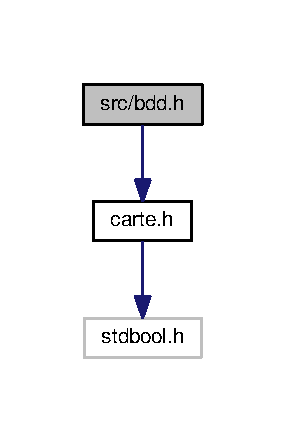
\includegraphics[width=137pt]{bdd_8h__incl}
\end{center}
\end{figure}
Ce graphe montre quels fichiers incluent directement ou indirectement ce fichier \+:\nopagebreak
\begin{figure}[H]
\begin{center}
\leavevmode
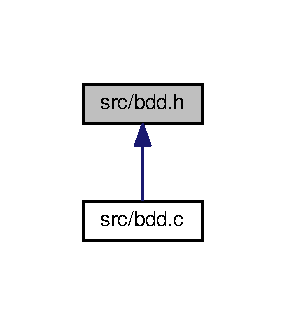
\includegraphics[width=137pt]{bdd_8h__dep__incl}
\end{center}
\end{figure}
\subsection*{Structures de données}
\begin{DoxyCompactItemize}
\item 
struct \hyperlink{structcarte__cell}{carte\+\_\+cell}
\begin{DoxyCompactList}\small\item\em Définit une cellule d\textquotesingle{}une liste chaînée de cartes. \end{DoxyCompactList}\item 
struct \hyperlink{structcarte__liste}{carte\+\_\+liste}
\begin{DoxyCompactList}\small\item\em Définit une liste chaînée de cartes. \end{DoxyCompactList}\end{DoxyCompactItemize}
\subsection*{Fonctions}
\begin{DoxyCompactItemize}
\item 
\hyperlink{structcarte__cell}{carte\+\_\+cell} $\ast$ \hyperlink{bdd_8h_a88fa0c6de52f3b77c0388812dd391c7d}{air\+\_\+bdd\+\_\+cell\+\_\+creer} (\hyperlink{structcarte}{carte} $\ast$c)
\begin{DoxyCompactList}\small\item\em Alloue et initialise une cellule. \end{DoxyCompactList}\item 
int \hyperlink{bdd_8h_a0042562c59847df384309d7f5ba2068d}{air\+\_\+bdd\+\_\+cell\+\_\+init} (\hyperlink{structcarte__cell}{carte\+\_\+cell} $\ast$cell, \hyperlink{structcarte}{carte} $\ast$c)
\begin{DoxyCompactList}\small\item\em Initialise une cellule. \end{DoxyCompactList}\item 
\hyperlink{structcarte__liste}{carte\+\_\+liste} $\ast$ \hyperlink{bdd_8h_a102d5682375fddae2f98591852922b10}{air\+\_\+bdd\+\_\+liste\+\_\+creer} ()
\begin{DoxyCompactList}\small\item\em Alloue et initialise une liste de cellules. \end{DoxyCompactList}\item 
int \hyperlink{bdd_8h_af35c055376980fd980cbc3e92df6cd7e}{air\+\_\+bdd\+\_\+liste\+\_\+init} (\hyperlink{structcarte__liste}{carte\+\_\+liste} $\ast$l)
\begin{DoxyCompactList}\small\item\em Initialise une liste de cellules. \end{DoxyCompactList}\item 
void \hyperlink{bdd_8h_a712e2dd20d20cc921237b8170af2fe52}{air\+\_\+bdd\+\_\+liste\+\_\+free} (\hyperlink{structcarte__liste}{carte\+\_\+liste} $\ast$l)
\begin{DoxyCompactList}\small\item\em Libère de la mémoire une liste de cellules. \end{DoxyCompactList}\item 
int \hyperlink{bdd_8h_a5fc0f20d939cef77b20fe0289cc28af3}{air\+\_\+bdd\+\_\+liste\+\_\+ajouter} (\hyperlink{structcarte__liste}{carte\+\_\+liste} $\ast$l, \hyperlink{structcarte}{carte} $\ast$c)
\begin{DoxyCompactList}\small\item\em Ajoute une carte à la liste. \end{DoxyCompactList}\item 
int \hyperlink{bdd_8h_adf6378260ec8d764e642fc89f7865f5f}{air\+\_\+bdd\+\_\+liste\+\_\+retirer} (\hyperlink{structcarte__liste}{carte\+\_\+liste} $\ast$l, \hyperlink{structcarte}{carte} $\ast$c)
\begin{DoxyCompactList}\small\item\em Reture une carte de la liste. \end{DoxyCompactList}\item 
int \hyperlink{bdd_8h_ab8e2391c7ec0afde492fc38ae88921fd}{air\+\_\+bdd\+\_\+liste\+\_\+taille} (\hyperlink{structcarte__liste}{carte\+\_\+liste} $\ast$l)
\begin{DoxyCompactList}\small\item\em Retourne la taille d\textquotesingle{}une liste de cartes. \end{DoxyCompactList}\item 
\hyperlink{structcarte__liste}{carte\+\_\+liste} $\ast$ \hyperlink{bdd_8h_ae69a985bbeb5d6c0abfb8449515b13e3}{air\+\_\+bdd\+\_\+liste\+\_\+recherche\+\_\+par\+\_\+valeur} (\hyperlink{structcarte__liste}{carte\+\_\+liste} $\ast$l, enum \hyperlink{carte_8h_a323916cdb68cd0d5d8a1660ffb45ea4e}{carte\+\_\+valeur} val)
\begin{DoxyCompactList}\small\item\em Retourne une liste des cartes ayant pour valeur {\ttfamily val} \end{DoxyCompactList}\item 
\hyperlink{structcarte__liste}{carte\+\_\+liste} $\ast$ \hyperlink{bdd_8h_ae342315c7c461f60b0830d40b8c80176}{air\+\_\+bdd\+\_\+liste\+\_\+recherche\+\_\+par\+\_\+enseigne} (\hyperlink{structcarte__liste}{carte\+\_\+liste} $\ast$l, enum \hyperlink{carte_8h_a2b6a5add5e3db9028dff54f9c1acdde7}{carte\+\_\+enseigne} enseigne)
\begin{DoxyCompactList}\small\item\em Retourne une liste des cartes ayant pour enseigne {\ttfamily enseigne} \end{DoxyCompactList}\item 
\hyperlink{structcarte__liste}{carte\+\_\+liste} $\ast$ \hyperlink{bdd_8h_a93cdadb2d656122f7a8c1f7f42278a9d}{air\+\_\+bdd\+\_\+liste\+\_\+recherche\+\_\+attaquants} (\hyperlink{structcarte__liste}{carte\+\_\+liste} $\ast$l, \hyperlink{structcarte}{carte} $\ast$c)
\begin{DoxyCompactList}\small\item\em Retourne la liste des cartes pouvant attaquer la carte {\ttfamily c} \end{DoxyCompactList}\item 
void \hyperlink{bdd_8h_a4f800054489e50ab8b51e876590b56df}{air\+\_\+bdd\+\_\+liste\+\_\+printf} (\hyperlink{structcarte__liste}{carte\+\_\+liste} $\ast$l)
\begin{DoxyCompactList}\small\item\em Affiche une liste de cartes sur la sortie standard. \end{DoxyCompactList}\end{DoxyCompactItemize}


\subsection{Description détaillée}
Définitions des fonctions de la base de données. 

\begin{DoxyAuthor}{Auteur}
Loïc Payol \href{mailto:loicpayol@gmail.com}{\tt loicpayol@gmail.\+com} 
\end{DoxyAuthor}


\subsection{Documentation des fonctions}
\index{bdd.\+h@{bdd.\+h}!air\+\_\+bdd\+\_\+cell\+\_\+creer@{air\+\_\+bdd\+\_\+cell\+\_\+creer}}
\index{air\+\_\+bdd\+\_\+cell\+\_\+creer@{air\+\_\+bdd\+\_\+cell\+\_\+creer}!bdd.\+h@{bdd.\+h}}
\subsubsection[{\texorpdfstring{air\+\_\+bdd\+\_\+cell\+\_\+creer(carte $\ast$c)}{air_bdd_cell_creer(carte *c)}}]{\setlength{\rightskip}{0pt plus 5cm}{\bf carte\+\_\+cell}$\ast$ air\+\_\+bdd\+\_\+cell\+\_\+creer (
\begin{DoxyParamCaption}
\item[{{\bf carte} $\ast$}]{c}
\end{DoxyParamCaption}
)}\hypertarget{bdd_8h_a88fa0c6de52f3b77c0388812dd391c7d}{}\label{bdd_8h_a88fa0c6de52f3b77c0388812dd391c7d}


Alloue et initialise une cellule. 


\begin{DoxyParams}{Paramètres}
{\em c} & La carte à encapsuler \\
\hline
\end{DoxyParams}
\begin{DoxyReturn}{Renvoie}
N\+U\+LL en cas d\textquotesingle{}erreur (voir errno), sinon la cellule nouvellement créée 
\end{DoxyReturn}
\index{bdd.\+h@{bdd.\+h}!air\+\_\+bdd\+\_\+cell\+\_\+init@{air\+\_\+bdd\+\_\+cell\+\_\+init}}
\index{air\+\_\+bdd\+\_\+cell\+\_\+init@{air\+\_\+bdd\+\_\+cell\+\_\+init}!bdd.\+h@{bdd.\+h}}
\subsubsection[{\texorpdfstring{air\+\_\+bdd\+\_\+cell\+\_\+init(carte\+\_\+cell $\ast$cell, carte $\ast$c)}{air_bdd_cell_init(carte_cell *cell, carte *c)}}]{\setlength{\rightskip}{0pt plus 5cm}int air\+\_\+bdd\+\_\+cell\+\_\+init (
\begin{DoxyParamCaption}
\item[{{\bf carte\+\_\+cell} $\ast$}]{cell, }
\item[{{\bf carte} $\ast$}]{c}
\end{DoxyParamCaption}
)}\hypertarget{bdd_8h_a0042562c59847df384309d7f5ba2068d}{}\label{bdd_8h_a0042562c59847df384309d7f5ba2068d}


Initialise une cellule. 


\begin{DoxyParams}{Paramètres}
{\em cell} & La cellule à initialiser \\
\hline
{\em c} & La carte à encapsuler \\
\hline
\end{DoxyParams}
\begin{DoxyReturn}{Renvoie}
-\/1 en cas d\textquotesingle{}erreur (voir errno), 0 sinon 
\end{DoxyReturn}
\index{bdd.\+h@{bdd.\+h}!air\+\_\+bdd\+\_\+liste\+\_\+ajouter@{air\+\_\+bdd\+\_\+liste\+\_\+ajouter}}
\index{air\+\_\+bdd\+\_\+liste\+\_\+ajouter@{air\+\_\+bdd\+\_\+liste\+\_\+ajouter}!bdd.\+h@{bdd.\+h}}
\subsubsection[{\texorpdfstring{air\+\_\+bdd\+\_\+liste\+\_\+ajouter(carte\+\_\+liste $\ast$l, carte $\ast$c)}{air_bdd_liste_ajouter(carte_liste *l, carte *c)}}]{\setlength{\rightskip}{0pt plus 5cm}int air\+\_\+bdd\+\_\+liste\+\_\+ajouter (
\begin{DoxyParamCaption}
\item[{{\bf carte\+\_\+liste} $\ast$}]{l, }
\item[{{\bf carte} $\ast$}]{c}
\end{DoxyParamCaption}
)}\hypertarget{bdd_8h_a5fc0f20d939cef77b20fe0289cc28af3}{}\label{bdd_8h_a5fc0f20d939cef77b20fe0289cc28af3}


Ajoute une carte à la liste. 


\begin{DoxyParams}{Paramètres}
{\em l} & La liste à manipuler \\
\hline
{\em c} & La carte à ajouter \\
\hline
\end{DoxyParams}
\begin{DoxyReturn}{Renvoie}
-\/1 en cas d\textquotesingle{}erreur (voir errno), 0 sinon 
\end{DoxyReturn}
\index{bdd.\+h@{bdd.\+h}!air\+\_\+bdd\+\_\+liste\+\_\+creer@{air\+\_\+bdd\+\_\+liste\+\_\+creer}}
\index{air\+\_\+bdd\+\_\+liste\+\_\+creer@{air\+\_\+bdd\+\_\+liste\+\_\+creer}!bdd.\+h@{bdd.\+h}}
\subsubsection[{\texorpdfstring{air\+\_\+bdd\+\_\+liste\+\_\+creer()}{air_bdd_liste_creer()}}]{\setlength{\rightskip}{0pt plus 5cm}{\bf carte\+\_\+liste}$\ast$ air\+\_\+bdd\+\_\+liste\+\_\+creer (
\begin{DoxyParamCaption}
{}
\end{DoxyParamCaption}
)}\hypertarget{bdd_8h_a102d5682375fddae2f98591852922b10}{}\label{bdd_8h_a102d5682375fddae2f98591852922b10}


Alloue et initialise une liste de cellules. 

\begin{DoxyReturn}{Renvoie}
N\+U\+LL en cas d\textquotesingle{}erreur (voir errno), sinon la liste nouvellement créée 
\end{DoxyReturn}
\index{bdd.\+h@{bdd.\+h}!air\+\_\+bdd\+\_\+liste\+\_\+free@{air\+\_\+bdd\+\_\+liste\+\_\+free}}
\index{air\+\_\+bdd\+\_\+liste\+\_\+free@{air\+\_\+bdd\+\_\+liste\+\_\+free}!bdd.\+h@{bdd.\+h}}
\subsubsection[{\texorpdfstring{air\+\_\+bdd\+\_\+liste\+\_\+free(carte\+\_\+liste $\ast$l)}{air_bdd_liste_free(carte_liste *l)}}]{\setlength{\rightskip}{0pt plus 5cm}void air\+\_\+bdd\+\_\+liste\+\_\+free (
\begin{DoxyParamCaption}
\item[{{\bf carte\+\_\+liste} $\ast$}]{l}
\end{DoxyParamCaption}
)}\hypertarget{bdd_8h_a712e2dd20d20cc921237b8170af2fe52}{}\label{bdd_8h_a712e2dd20d20cc921237b8170af2fe52}


Libère de la mémoire une liste de cellules. 


\begin{DoxyParams}{Paramètres}
{\em l} & La liste à libérer de la mémoire \\
\hline
\end{DoxyParams}
\index{bdd.\+h@{bdd.\+h}!air\+\_\+bdd\+\_\+liste\+\_\+init@{air\+\_\+bdd\+\_\+liste\+\_\+init}}
\index{air\+\_\+bdd\+\_\+liste\+\_\+init@{air\+\_\+bdd\+\_\+liste\+\_\+init}!bdd.\+h@{bdd.\+h}}
\subsubsection[{\texorpdfstring{air\+\_\+bdd\+\_\+liste\+\_\+init(carte\+\_\+liste $\ast$l)}{air_bdd_liste_init(carte_liste *l)}}]{\setlength{\rightskip}{0pt plus 5cm}int air\+\_\+bdd\+\_\+liste\+\_\+init (
\begin{DoxyParamCaption}
\item[{{\bf carte\+\_\+liste} $\ast$}]{l}
\end{DoxyParamCaption}
)}\hypertarget{bdd_8h_af35c055376980fd980cbc3e92df6cd7e}{}\label{bdd_8h_af35c055376980fd980cbc3e92df6cd7e}


Initialise une liste de cellules. 


\begin{DoxyParams}{Paramètres}
{\em l} & La liste à initialiser \\
\hline
\end{DoxyParams}
\begin{DoxyReturn}{Renvoie}
-\/1 en cas d\textquotesingle{}erreur (voir errno), 0 sinon 
\end{DoxyReturn}
\index{bdd.\+h@{bdd.\+h}!air\+\_\+bdd\+\_\+liste\+\_\+printf@{air\+\_\+bdd\+\_\+liste\+\_\+printf}}
\index{air\+\_\+bdd\+\_\+liste\+\_\+printf@{air\+\_\+bdd\+\_\+liste\+\_\+printf}!bdd.\+h@{bdd.\+h}}
\subsubsection[{\texorpdfstring{air\+\_\+bdd\+\_\+liste\+\_\+printf(carte\+\_\+liste $\ast$l)}{air_bdd_liste_printf(carte_liste *l)}}]{\setlength{\rightskip}{0pt plus 5cm}void air\+\_\+bdd\+\_\+liste\+\_\+printf (
\begin{DoxyParamCaption}
\item[{{\bf carte\+\_\+liste} $\ast$}]{l}
\end{DoxyParamCaption}
)}\hypertarget{bdd_8h_a4f800054489e50ab8b51e876590b56df}{}\label{bdd_8h_a4f800054489e50ab8b51e876590b56df}


Affiche une liste de cartes sur la sortie standard. 


\begin{DoxyParams}{Paramètres}
{\em l} & La liste à afficher \\
\hline
\end{DoxyParams}
\index{bdd.\+h@{bdd.\+h}!air\+\_\+bdd\+\_\+liste\+\_\+recherche\+\_\+attaquants@{air\+\_\+bdd\+\_\+liste\+\_\+recherche\+\_\+attaquants}}
\index{air\+\_\+bdd\+\_\+liste\+\_\+recherche\+\_\+attaquants@{air\+\_\+bdd\+\_\+liste\+\_\+recherche\+\_\+attaquants}!bdd.\+h@{bdd.\+h}}
\subsubsection[{\texorpdfstring{air\+\_\+bdd\+\_\+liste\+\_\+recherche\+\_\+attaquants(carte\+\_\+liste $\ast$l, carte $\ast$c)}{air_bdd_liste_recherche_attaquants(carte_liste *l, carte *c)}}]{\setlength{\rightskip}{0pt plus 5cm}{\bf carte\+\_\+liste}$\ast$ air\+\_\+bdd\+\_\+liste\+\_\+recherche\+\_\+attaquants (
\begin{DoxyParamCaption}
\item[{{\bf carte\+\_\+liste} $\ast$}]{l, }
\item[{{\bf carte} $\ast$}]{c}
\end{DoxyParamCaption}
)}\hypertarget{bdd_8h_a93cdadb2d656122f7a8c1f7f42278a9d}{}\label{bdd_8h_a93cdadb2d656122f7a8c1f7f42278a9d}


Retourne la liste des cartes pouvant attaquer la carte {\ttfamily c} 


\begin{DoxyParams}{Paramètres}
{\em l} & La liste sur laquelle effectuer la recherche \\
\hline
{\em c} & La carte \char`\"{}attaquée\char`\"{} \\
\hline
\end{DoxyParams}
\begin{DoxyReturn}{Renvoie}
N\+U\+LL en cas d\textquotesingle{}erreur (voir errno), sinon retourne la liste résultat 
\end{DoxyReturn}
\index{bdd.\+h@{bdd.\+h}!air\+\_\+bdd\+\_\+liste\+\_\+recherche\+\_\+par\+\_\+enseigne@{air\+\_\+bdd\+\_\+liste\+\_\+recherche\+\_\+par\+\_\+enseigne}}
\index{air\+\_\+bdd\+\_\+liste\+\_\+recherche\+\_\+par\+\_\+enseigne@{air\+\_\+bdd\+\_\+liste\+\_\+recherche\+\_\+par\+\_\+enseigne}!bdd.\+h@{bdd.\+h}}
\subsubsection[{\texorpdfstring{air\+\_\+bdd\+\_\+liste\+\_\+recherche\+\_\+par\+\_\+enseigne(carte\+\_\+liste $\ast$l, enum carte\+\_\+enseigne enseigne)}{air_bdd_liste_recherche_par_enseigne(carte_liste *l, enum carte_enseigne enseigne)}}]{\setlength{\rightskip}{0pt plus 5cm}{\bf carte\+\_\+liste}$\ast$ air\+\_\+bdd\+\_\+liste\+\_\+recherche\+\_\+par\+\_\+enseigne (
\begin{DoxyParamCaption}
\item[{{\bf carte\+\_\+liste} $\ast$}]{l, }
\item[{enum {\bf carte\+\_\+enseigne}}]{enseigne}
\end{DoxyParamCaption}
)}\hypertarget{bdd_8h_ae342315c7c461f60b0830d40b8c80176}{}\label{bdd_8h_ae342315c7c461f60b0830d40b8c80176}


Retourne une liste des cartes ayant pour enseigne {\ttfamily enseigne} 


\begin{DoxyParams}{Paramètres}
{\em l} & La liste sur laquelle exécuter la requête (allouée dynamiquement) \\
\hline
{\em enseigne} & L\textquotesingle{}enseigne à rechercher \\
\hline
\end{DoxyParams}
\begin{DoxyReturn}{Renvoie}
N\+U\+LL en cas d\textquotesingle{}erreur (voir errno), sinon retourne la liste résultat 
\end{DoxyReturn}
\index{bdd.\+h@{bdd.\+h}!air\+\_\+bdd\+\_\+liste\+\_\+recherche\+\_\+par\+\_\+valeur@{air\+\_\+bdd\+\_\+liste\+\_\+recherche\+\_\+par\+\_\+valeur}}
\index{air\+\_\+bdd\+\_\+liste\+\_\+recherche\+\_\+par\+\_\+valeur@{air\+\_\+bdd\+\_\+liste\+\_\+recherche\+\_\+par\+\_\+valeur}!bdd.\+h@{bdd.\+h}}
\subsubsection[{\texorpdfstring{air\+\_\+bdd\+\_\+liste\+\_\+recherche\+\_\+par\+\_\+valeur(carte\+\_\+liste $\ast$l, enum carte\+\_\+valeur val)}{air_bdd_liste_recherche_par_valeur(carte_liste *l, enum carte_valeur val)}}]{\setlength{\rightskip}{0pt plus 5cm}{\bf carte\+\_\+liste}$\ast$ air\+\_\+bdd\+\_\+liste\+\_\+recherche\+\_\+par\+\_\+valeur (
\begin{DoxyParamCaption}
\item[{{\bf carte\+\_\+liste} $\ast$}]{l, }
\item[{enum {\bf carte\+\_\+valeur}}]{val}
\end{DoxyParamCaption}
)}\hypertarget{bdd_8h_ae69a985bbeb5d6c0abfb8449515b13e3}{}\label{bdd_8h_ae69a985bbeb5d6c0abfb8449515b13e3}


Retourne une liste des cartes ayant pour valeur {\ttfamily val} 


\begin{DoxyParams}{Paramètres}
{\em l} & La liste sur laquelle exécuter la requête (allouée dynamiquement) \\
\hline
{\em val} & La valeur à rechercher \\
\hline
\end{DoxyParams}
\begin{DoxyReturn}{Renvoie}
N\+U\+LL en cas d\textquotesingle{}erreur (voir errno), sinon retourne la liste résultat 
\end{DoxyReturn}
\index{bdd.\+h@{bdd.\+h}!air\+\_\+bdd\+\_\+liste\+\_\+retirer@{air\+\_\+bdd\+\_\+liste\+\_\+retirer}}
\index{air\+\_\+bdd\+\_\+liste\+\_\+retirer@{air\+\_\+bdd\+\_\+liste\+\_\+retirer}!bdd.\+h@{bdd.\+h}}
\subsubsection[{\texorpdfstring{air\+\_\+bdd\+\_\+liste\+\_\+retirer(carte\+\_\+liste $\ast$l, carte $\ast$c)}{air_bdd_liste_retirer(carte_liste *l, carte *c)}}]{\setlength{\rightskip}{0pt plus 5cm}int air\+\_\+bdd\+\_\+liste\+\_\+retirer (
\begin{DoxyParamCaption}
\item[{{\bf carte\+\_\+liste} $\ast$}]{l, }
\item[{{\bf carte} $\ast$}]{c}
\end{DoxyParamCaption}
)}\hypertarget{bdd_8h_adf6378260ec8d764e642fc89f7865f5f}{}\label{bdd_8h_adf6378260ec8d764e642fc89f7865f5f}


Reture une carte de la liste. 


\begin{DoxyParams}{Paramètres}
{\em l} & La liste à manipuler \\
\hline
{\em c} & La carte à retirer \\
\hline
\end{DoxyParams}
\begin{DoxyReturn}{Renvoie}
-\/1 en cas d\textquotesingle{}erreur (voir errno), 0 si l\textquotesingle{}élément a été retiré, 1 si l\textquotesingle{}élément n\textquotesingle{}était pas dans la liste 
\end{DoxyReturn}
\index{bdd.\+h@{bdd.\+h}!air\+\_\+bdd\+\_\+liste\+\_\+taille@{air\+\_\+bdd\+\_\+liste\+\_\+taille}}
\index{air\+\_\+bdd\+\_\+liste\+\_\+taille@{air\+\_\+bdd\+\_\+liste\+\_\+taille}!bdd.\+h@{bdd.\+h}}
\subsubsection[{\texorpdfstring{air\+\_\+bdd\+\_\+liste\+\_\+taille(carte\+\_\+liste $\ast$l)}{air_bdd_liste_taille(carte_liste *l)}}]{\setlength{\rightskip}{0pt plus 5cm}int air\+\_\+bdd\+\_\+liste\+\_\+taille (
\begin{DoxyParamCaption}
\item[{{\bf carte\+\_\+liste} $\ast$}]{l}
\end{DoxyParamCaption}
)}\hypertarget{bdd_8h_ab8e2391c7ec0afde492fc38ae88921fd}{}\label{bdd_8h_ab8e2391c7ec0afde492fc38ae88921fd}


Retourne la taille d\textquotesingle{}une liste de cartes. 


\begin{DoxyParams}{Paramètres}
{\em l} & La liste de cartes à manipuler \\
\hline
\end{DoxyParams}
\begin{DoxyReturn}{Renvoie}
-\/1 en cas d\textquotesingle{}erreur (voir errno), sinon la taille de la liste 
\end{DoxyReturn}

\hypertarget{carte_8c}{}\section{Référence du fichier src/carte.c}
\label{carte_8c}\index{src/carte.\+c@{src/carte.\+c}}


Fonctions de manipulation de l\textquotesingle{}entité \char`\"{}carte\char`\"{}.  


{\ttfamily \#include $<$stdlib.\+h$>$}\\*
{\ttfamily \#include $<$stdio.\+h$>$}\\*
{\ttfamily \#include $<$errno.\+h$>$}\\*
{\ttfamily \#include \char`\"{}carte.\+h\char`\"{}}\\*
Graphe des dépendances par inclusion de carte.\+c\+:\nopagebreak
\begin{figure}[H]
\begin{center}
\leavevmode
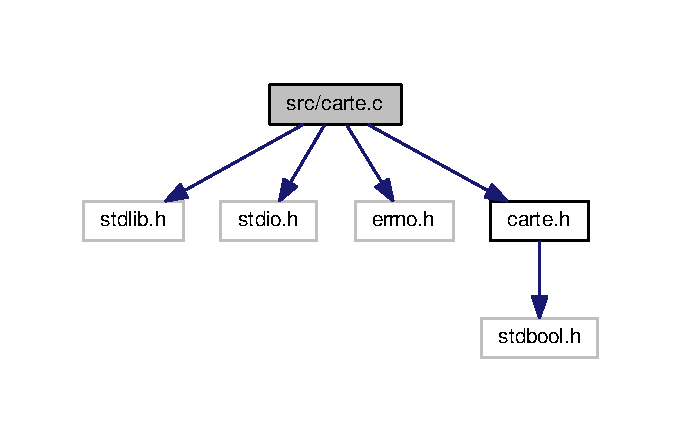
\includegraphics[width=327pt]{carte_8c__incl}
\end{center}
\end{figure}
\subsection*{Fonctions}
\begin{DoxyCompactItemize}
\item 
\hyperlink{structcarte}{carte} $\ast$ \hyperlink{carte_8c_af0ff4aff78039e6842dc705c6ad19f3d}{air\+\_\+carte\+\_\+creer} ()
\begin{DoxyCompactList}\small\item\em Alloue dynamiquement une carte et l\textquotesingle{}initialise. \end{DoxyCompactList}\item 
void \hyperlink{carte_8c_a45274a3996ff9bed9e3d6e978655a1d4}{air\+\_\+carte\+\_\+free} (\hyperlink{structcarte}{carte} $\ast$c)
\begin{DoxyCompactList}\small\item\em Libère de la mémoire une carte. \end{DoxyCompactList}\item 
\hyperlink{structcarte__prop}{carte\+\_\+prop} $\ast$ \hyperlink{carte_8c_ad8931bfc61291dbc9a929cd957c998ee}{air\+\_\+carte\+\_\+prop\+\_\+creer} ()
\begin{DoxyCompactList}\small\item\em Alloue la mémoire pour une \hyperlink{structcarte__prop}{carte\+\_\+prop} et l\textquotesingle{}initialise. \end{DoxyCompactList}\item 
int \hyperlink{carte_8c_a1841a8f25ee0e8f4ee53f84b383772e4}{air\+\_\+carte\+\_\+prop\+\_\+init} (\hyperlink{structcarte__prop}{carte\+\_\+prop} $\ast$p)
\begin{DoxyCompactList}\small\item\em Initialise une \hyperlink{structcarte__prop}{carte\+\_\+prop}. \end{DoxyCompactList}\item 
\hyperlink{structcarte__prop}{carte\+\_\+prop} $\ast$ \hyperlink{carte_8c_aaa719861c5e04eac040e825975ad04d4}{air\+\_\+carte\+\_\+prop\+\_\+find\+\_\+type} (\hyperlink{structcarte__prop}{carte\+\_\+prop} $\ast$ptr, enum \hyperlink{carte_8h_a71a2818c25230a5e1a239f28c1e6deba}{carte\+\_\+prop\+\_\+type} type)
\begin{DoxyCompactList}\small\item\em Recherche la première propriété de type {\ttfamily type} dans la chaîne des propriétés d\textquotesingle{}une carte donnée. \end{DoxyCompactList}\item 
int \hyperlink{carte_8c_ab931f47e29ed5f74a4b24f35503af391}{air\+\_\+carte\+\_\+prop\+\_\+ajouter} (\hyperlink{structcarte}{carte} $\ast$c, \hyperlink{structcarte__prop}{carte\+\_\+prop} $\ast$p)
\begin{DoxyCompactList}\small\item\em Ajoute une propriété à la carte. \end{DoxyCompactList}\item 
int \hyperlink{carte_8c_aca47330fc7b74166365ab3aea4d303a1}{air\+\_\+carte\+\_\+init} (\hyperlink{structcarte}{carte} $\ast$c)
\begin{DoxyCompactList}\small\item\em Initialise la structure. \end{DoxyCompactList}\item 
enum \hyperlink{carte_8h_a323916cdb68cd0d5d8a1660ffb45ea4e}{carte\+\_\+valeur} \hyperlink{carte_8c_ab411344f241870ba183d6c5db6c4898b}{air\+\_\+carte\+\_\+valeur\+\_\+get} (\hyperlink{structcarte}{carte} $\ast$c)
\begin{DoxyCompactList}\small\item\em Retourne la valeur d\textquotesingle{}une carte. \end{DoxyCompactList}\item 
int \hyperlink{carte_8c_addfb4cc8cdc67446e1fb2434bdbec2d0}{air\+\_\+carte\+\_\+valeur\+\_\+set} (\hyperlink{structcarte}{carte} $\ast$c, enum \hyperlink{carte_8h_a323916cdb68cd0d5d8a1660ffb45ea4e}{carte\+\_\+valeur} valeur)
\begin{DoxyCompactList}\small\item\em Affecte la valeur {\ttfamily valeur} à la carte. \end{DoxyCompactList}\item 
enum \hyperlink{carte_8h_a2b6a5add5e3db9028dff54f9c1acdde7}{carte\+\_\+enseigne} \hyperlink{carte_8c_a7dad267d5ce0603d60ddd72230aadc46}{air\+\_\+carte\+\_\+enseigne\+\_\+get} (\hyperlink{structcarte}{carte} $\ast$c)
\begin{DoxyCompactList}\small\item\em Retourne l\textquotesingle{}enseigne d\textquotesingle{}une carte. \end{DoxyCompactList}\item 
int \hyperlink{carte_8c_ad4dda778eb53e034326b558828cf2a40}{air\+\_\+carte\+\_\+enseigne\+\_\+set} (\hyperlink{structcarte}{carte} $\ast$c, enum \hyperlink{carte_8h_a2b6a5add5e3db9028dff54f9c1acdde7}{carte\+\_\+enseigne} enseigne)
\begin{DoxyCompactList}\small\item\em Affecte l\textquotesingle{}enseigne {\ttfamily enseigne} à la carte. \end{DoxyCompactList}\item 
bool \hyperlink{carte_8c_ad7eae524fba5e88efa3d7862655dd8df}{air\+\_\+carte\+\_\+peut\+\_\+battre} (\hyperlink{structcarte}{carte} $\ast$c, \hyperlink{structcarte}{carte} $\ast$peut\+\_\+battre)
\begin{DoxyCompactList}\small\item\em Vérifie si une carte peut en battre une autre. \end{DoxyCompactList}\item 
int \hyperlink{carte_8c_a63216eb2cdd6219203225de97f47c251}{air\+\_\+carte\+\_\+bat\+\_\+add} (\hyperlink{structcarte}{carte} $\ast$c, \hyperlink{structcarte}{carte} $\ast$peut\+\_\+battre)
\begin{DoxyCompactList}\small\item\em Affecte à une carte une référence vers une autre carte. \end{DoxyCompactList}\item 
void \hyperlink{carte_8c_ac6c44bf3c40f97468e22dcebfb622a6b}{air\+\_\+carte\+\_\+printf} (\hyperlink{structcarte}{carte} $\ast$c)
\begin{DoxyCompactList}\small\item\em Affiche les propriétés d\textquotesingle{}une carte sur la sortie standard. \end{DoxyCompactList}\item 
void \hyperlink{carte_8c_ae6ffa5f0d892f4d19b569f4ebc46564e}{air\+\_\+carte\+\_\+affiche\+\_\+valeur} (enum \hyperlink{carte_8h_a323916cdb68cd0d5d8a1660ffb45ea4e}{carte\+\_\+valeur} valeur)
\begin{DoxyCompactList}\small\item\em Affiche la valeur passée en paramètre dans la sortie standard. \end{DoxyCompactList}\item 
void \hyperlink{carte_8c_aa5514ebef2fa8a1d26628f153c3768e8}{air\+\_\+carte\+\_\+affiche\+\_\+enseigne} (enum \hyperlink{carte_8h_a2b6a5add5e3db9028dff54f9c1acdde7}{carte\+\_\+enseigne} enseigne)
\begin{DoxyCompactList}\small\item\em Affiche l\textquotesingle{}enseigne passée en paramètre dans la sortie standard. \end{DoxyCompactList}\end{DoxyCompactItemize}


\subsection{Description détaillée}
Fonctions de manipulation de l\textquotesingle{}entité \char`\"{}carte\char`\"{}. 

\begin{DoxyAuthor}{Auteur}
Loïc Payol \href{mailto:loicpayol@gmail.com}{\tt loicpayol@gmail.\+com} 
\end{DoxyAuthor}


\subsection{Documentation des fonctions}
\index{carte.\+c@{carte.\+c}!air\+\_\+carte\+\_\+affiche\+\_\+enseigne@{air\+\_\+carte\+\_\+affiche\+\_\+enseigne}}
\index{air\+\_\+carte\+\_\+affiche\+\_\+enseigne@{air\+\_\+carte\+\_\+affiche\+\_\+enseigne}!carte.\+c@{carte.\+c}}
\subsubsection[{\texorpdfstring{air\+\_\+carte\+\_\+affiche\+\_\+enseigne(enum carte\+\_\+enseigne enseigne)}{air_carte_affiche_enseigne(enum carte_enseigne enseigne)}}]{\setlength{\rightskip}{0pt plus 5cm}void air\+\_\+carte\+\_\+affiche\+\_\+enseigne (
\begin{DoxyParamCaption}
\item[{enum {\bf carte\+\_\+enseigne}}]{enseigne}
\end{DoxyParamCaption}
)}\hypertarget{carte_8c_aa5514ebef2fa8a1d26628f153c3768e8}{}\label{carte_8c_aa5514ebef2fa8a1d26628f153c3768e8}


Affiche l\textquotesingle{}enseigne passée en paramètre dans la sortie standard. 


\begin{DoxyParams}{Paramètres}
{\em valeur} & L\textquotesingle{}enseigne à afficher \\
\hline
\end{DoxyParams}
\index{carte.\+c@{carte.\+c}!air\+\_\+carte\+\_\+affiche\+\_\+valeur@{air\+\_\+carte\+\_\+affiche\+\_\+valeur}}
\index{air\+\_\+carte\+\_\+affiche\+\_\+valeur@{air\+\_\+carte\+\_\+affiche\+\_\+valeur}!carte.\+c@{carte.\+c}}
\subsubsection[{\texorpdfstring{air\+\_\+carte\+\_\+affiche\+\_\+valeur(enum carte\+\_\+valeur valeur)}{air_carte_affiche_valeur(enum carte_valeur valeur)}}]{\setlength{\rightskip}{0pt plus 5cm}void air\+\_\+carte\+\_\+affiche\+\_\+valeur (
\begin{DoxyParamCaption}
\item[{enum {\bf carte\+\_\+valeur}}]{valeur}
\end{DoxyParamCaption}
)}\hypertarget{carte_8c_ae6ffa5f0d892f4d19b569f4ebc46564e}{}\label{carte_8c_ae6ffa5f0d892f4d19b569f4ebc46564e}


Affiche la valeur passée en paramètre dans la sortie standard. 


\begin{DoxyParams}{Paramètres}
{\em valeur} & La valeur à afficher \\
\hline
\end{DoxyParams}
\index{carte.\+c@{carte.\+c}!air\+\_\+carte\+\_\+bat\+\_\+add@{air\+\_\+carte\+\_\+bat\+\_\+add}}
\index{air\+\_\+carte\+\_\+bat\+\_\+add@{air\+\_\+carte\+\_\+bat\+\_\+add}!carte.\+c@{carte.\+c}}
\subsubsection[{\texorpdfstring{air\+\_\+carte\+\_\+bat\+\_\+add(carte $\ast$c, carte $\ast$peut\+\_\+battre)}{air_carte_bat_add(carte *c, carte *peut_battre)}}]{\setlength{\rightskip}{0pt plus 5cm}int air\+\_\+carte\+\_\+bat\+\_\+add (
\begin{DoxyParamCaption}
\item[{{\bf carte} $\ast$}]{c, }
\item[{{\bf carte} $\ast$}]{peut\+\_\+battre}
\end{DoxyParamCaption}
)}\hypertarget{carte_8c_a63216eb2cdd6219203225de97f47c251}{}\label{carte_8c_a63216eb2cdd6219203225de97f47c251}


Affecte à une carte une référence vers une autre carte. 


\begin{DoxyParams}{Paramètres}
{\em c} & L\textquotesingle{}instance de la structure à modifier \\
\hline
{\em peut\+\_\+battre} & La carte battue \\
\hline
\end{DoxyParams}
\begin{DoxyReturn}{Renvoie}
0 lorsqu\textquotesingle{}aucune erreur n\textquotesingle{}a eu lieu, -\/1 quand une erreur a eu lieu (peut\+\_\+battre == N\+U\+LL ou à c) 
\end{DoxyReturn}
\index{carte.\+c@{carte.\+c}!air\+\_\+carte\+\_\+creer@{air\+\_\+carte\+\_\+creer}}
\index{air\+\_\+carte\+\_\+creer@{air\+\_\+carte\+\_\+creer}!carte.\+c@{carte.\+c}}
\subsubsection[{\texorpdfstring{air\+\_\+carte\+\_\+creer()}{air_carte_creer()}}]{\setlength{\rightskip}{0pt plus 5cm}{\bf carte} $\ast$ air\+\_\+carte\+\_\+creer (
\begin{DoxyParamCaption}
{}
\end{DoxyParamCaption}
)}\hypertarget{carte_8c_af0ff4aff78039e6842dc705c6ad19f3d}{}\label{carte_8c_af0ff4aff78039e6842dc705c6ad19f3d}


Alloue dynamiquement une carte et l\textquotesingle{}initialise. 

\begin{DoxyReturn}{Renvoie}
N\+U\+LL en cas d\textquotesingle{}erreur (voir errno), sinon la carte nouvellement créée 
\end{DoxyReturn}
\index{carte.\+c@{carte.\+c}!air\+\_\+carte\+\_\+enseigne\+\_\+get@{air\+\_\+carte\+\_\+enseigne\+\_\+get}}
\index{air\+\_\+carte\+\_\+enseigne\+\_\+get@{air\+\_\+carte\+\_\+enseigne\+\_\+get}!carte.\+c@{carte.\+c}}
\subsubsection[{\texorpdfstring{air\+\_\+carte\+\_\+enseigne\+\_\+get(carte $\ast$c)}{air_carte_enseigne_get(carte *c)}}]{\setlength{\rightskip}{0pt plus 5cm}enum {\bf carte\+\_\+enseigne} air\+\_\+carte\+\_\+enseigne\+\_\+get (
\begin{DoxyParamCaption}
\item[{{\bf carte} $\ast$}]{c}
\end{DoxyParamCaption}
)}\hypertarget{carte_8c_a7dad267d5ce0603d60ddd72230aadc46}{}\label{carte_8c_a7dad267d5ce0603d60ddd72230aadc46}


Retourne l\textquotesingle{}enseigne d\textquotesingle{}une carte. 


\begin{DoxyParams}{Paramètres}
{\em c} & La carte \\
\hline
\end{DoxyParams}
\begin{DoxyReturn}{Renvoie}
L\textquotesingle{}enseigne de la carte 
\end{DoxyReturn}
\index{carte.\+c@{carte.\+c}!air\+\_\+carte\+\_\+enseigne\+\_\+set@{air\+\_\+carte\+\_\+enseigne\+\_\+set}}
\index{air\+\_\+carte\+\_\+enseigne\+\_\+set@{air\+\_\+carte\+\_\+enseigne\+\_\+set}!carte.\+c@{carte.\+c}}
\subsubsection[{\texorpdfstring{air\+\_\+carte\+\_\+enseigne\+\_\+set(carte $\ast$c, enum carte\+\_\+enseigne enseigne)}{air_carte_enseigne_set(carte *c, enum carte_enseigne enseigne)}}]{\setlength{\rightskip}{0pt plus 5cm}int air\+\_\+carte\+\_\+enseigne\+\_\+set (
\begin{DoxyParamCaption}
\item[{{\bf carte} $\ast$}]{c, }
\item[{enum {\bf carte\+\_\+enseigne}}]{enseigne}
\end{DoxyParamCaption}
)}\hypertarget{carte_8c_ad4dda778eb53e034326b558828cf2a40}{}\label{carte_8c_ad4dda778eb53e034326b558828cf2a40}


Affecte l\textquotesingle{}enseigne {\ttfamily enseigne} à la carte. 


\begin{DoxyParams}{Paramètres}
{\em c} & L\textquotesingle{}instance de la structure à modifier \\
\hline
{\em enseigne} & L\textquotesingle{}enseigne à affecter \\
\hline
\end{DoxyParams}
\begin{DoxyReturn}{Renvoie}
0 lorsqu\textquotesingle{}aucune erreur n\textquotesingle{}a eu lieu 
\end{DoxyReturn}
\index{carte.\+c@{carte.\+c}!air\+\_\+carte\+\_\+free@{air\+\_\+carte\+\_\+free}}
\index{air\+\_\+carte\+\_\+free@{air\+\_\+carte\+\_\+free}!carte.\+c@{carte.\+c}}
\subsubsection[{\texorpdfstring{air\+\_\+carte\+\_\+free(carte $\ast$c)}{air_carte_free(carte *c)}}]{\setlength{\rightskip}{0pt plus 5cm}void air\+\_\+carte\+\_\+free (
\begin{DoxyParamCaption}
\item[{{\bf carte} $\ast$}]{c}
\end{DoxyParamCaption}
)}\hypertarget{carte_8c_a45274a3996ff9bed9e3d6e978655a1d4}{}\label{carte_8c_a45274a3996ff9bed9e3d6e978655a1d4}


Libère de la mémoire une carte. 


\begin{DoxyParams}{Paramètres}
{\em c} & La carte à libérer de la mémoire \\
\hline
\end{DoxyParams}
\index{carte.\+c@{carte.\+c}!air\+\_\+carte\+\_\+init@{air\+\_\+carte\+\_\+init}}
\index{air\+\_\+carte\+\_\+init@{air\+\_\+carte\+\_\+init}!carte.\+c@{carte.\+c}}
\subsubsection[{\texorpdfstring{air\+\_\+carte\+\_\+init(carte $\ast$c)}{air_carte_init(carte *c)}}]{\setlength{\rightskip}{0pt plus 5cm}int air\+\_\+carte\+\_\+init (
\begin{DoxyParamCaption}
\item[{{\bf carte} $\ast$}]{c}
\end{DoxyParamCaption}
)}\hypertarget{carte_8c_aca47330fc7b74166365ab3aea4d303a1}{}\label{carte_8c_aca47330fc7b74166365ab3aea4d303a1}


Initialise la structure. 


\begin{DoxyParams}{Paramètres}
{\em c} & L\textquotesingle{}instance de la structure à initialiser \\
\hline
\end{DoxyParams}
\begin{DoxyReturn}{Renvoie}
0 lorsqu\textquotesingle{}aucune erreur n\textquotesingle{}a eu lieu 
\end{DoxyReturn}
\index{carte.\+c@{carte.\+c}!air\+\_\+carte\+\_\+peut\+\_\+battre@{air\+\_\+carte\+\_\+peut\+\_\+battre}}
\index{air\+\_\+carte\+\_\+peut\+\_\+battre@{air\+\_\+carte\+\_\+peut\+\_\+battre}!carte.\+c@{carte.\+c}}
\subsubsection[{\texorpdfstring{air\+\_\+carte\+\_\+peut\+\_\+battre(carte $\ast$c, carte $\ast$peut\+\_\+battre)}{air_carte_peut_battre(carte *c, carte *peut_battre)}}]{\setlength{\rightskip}{0pt plus 5cm}bool air\+\_\+carte\+\_\+peut\+\_\+battre (
\begin{DoxyParamCaption}
\item[{{\bf carte} $\ast$}]{c, }
\item[{{\bf carte} $\ast$}]{peut\+\_\+battre}
\end{DoxyParamCaption}
)}\hypertarget{carte_8c_ad7eae524fba5e88efa3d7862655dd8df}{}\label{carte_8c_ad7eae524fba5e88efa3d7862655dd8df}


Vérifie si une carte peut en battre une autre. 


\begin{DoxyParams}{Paramètres}
{\em c} & La carte \char`\"{}attaquante\char`\"{} \\
\hline
{\em peut\+\_\+battre} & La carte \char`\"{}attaquée\char`\"{} \\
\hline
\end{DoxyParams}
\begin{DoxyReturn}{Renvoie}
true si la carte attaquante peut la battre, false sinon 
\end{DoxyReturn}
\index{carte.\+c@{carte.\+c}!air\+\_\+carte\+\_\+printf@{air\+\_\+carte\+\_\+printf}}
\index{air\+\_\+carte\+\_\+printf@{air\+\_\+carte\+\_\+printf}!carte.\+c@{carte.\+c}}
\subsubsection[{\texorpdfstring{air\+\_\+carte\+\_\+printf(carte $\ast$c)}{air_carte_printf(carte *c)}}]{\setlength{\rightskip}{0pt plus 5cm}void air\+\_\+carte\+\_\+printf (
\begin{DoxyParamCaption}
\item[{{\bf carte} $\ast$}]{c}
\end{DoxyParamCaption}
)}\hypertarget{carte_8c_ac6c44bf3c40f97468e22dcebfb622a6b}{}\label{carte_8c_ac6c44bf3c40f97468e22dcebfb622a6b}


Affiche les propriétés d\textquotesingle{}une carte sur la sortie standard. 


\begin{DoxyParams}{Paramètres}
{\em c} & La carte à afficher \\
\hline
\end{DoxyParams}
\index{carte.\+c@{carte.\+c}!air\+\_\+carte\+\_\+prop\+\_\+ajouter@{air\+\_\+carte\+\_\+prop\+\_\+ajouter}}
\index{air\+\_\+carte\+\_\+prop\+\_\+ajouter@{air\+\_\+carte\+\_\+prop\+\_\+ajouter}!carte.\+c@{carte.\+c}}
\subsubsection[{\texorpdfstring{air\+\_\+carte\+\_\+prop\+\_\+ajouter(carte $\ast$c, carte\+\_\+prop $\ast$p)}{air_carte_prop_ajouter(carte *c, carte_prop *p)}}]{\setlength{\rightskip}{0pt plus 5cm}int air\+\_\+carte\+\_\+prop\+\_\+ajouter (
\begin{DoxyParamCaption}
\item[{{\bf carte} $\ast$}]{c, }
\item[{{\bf carte\+\_\+prop} $\ast$}]{p}
\end{DoxyParamCaption}
)}\hypertarget{carte_8c_ab931f47e29ed5f74a4b24f35503af391}{}\label{carte_8c_ab931f47e29ed5f74a4b24f35503af391}


Ajoute une propriété à la carte. 


\begin{DoxyParams}{Paramètres}
{\em c} & La carte à modifier \\
\hline
{\em p} & La propriété à ajouter \\
\hline
\end{DoxyParams}
\begin{DoxyReturn}{Renvoie}
0 lorsqu\textquotesingle{}aucune erreur n\textquotesingle{}a eu lieu 
\end{DoxyReturn}
\index{carte.\+c@{carte.\+c}!air\+\_\+carte\+\_\+prop\+\_\+creer@{air\+\_\+carte\+\_\+prop\+\_\+creer}}
\index{air\+\_\+carte\+\_\+prop\+\_\+creer@{air\+\_\+carte\+\_\+prop\+\_\+creer}!carte.\+c@{carte.\+c}}
\subsubsection[{\texorpdfstring{air\+\_\+carte\+\_\+prop\+\_\+creer()}{air_carte_prop_creer()}}]{\setlength{\rightskip}{0pt plus 5cm}{\bf carte\+\_\+prop} $\ast$ air\+\_\+carte\+\_\+prop\+\_\+creer (
\begin{DoxyParamCaption}
{}
\end{DoxyParamCaption}
)}\hypertarget{carte_8c_ad8931bfc61291dbc9a929cd957c998ee}{}\label{carte_8c_ad8931bfc61291dbc9a929cd957c998ee}


Alloue la mémoire pour une \hyperlink{structcarte__prop}{carte\+\_\+prop} et l\textquotesingle{}initialise. 

\begin{DoxyReturn}{Renvoie}
N\+U\+LL en cas d\textquotesingle{}erreur (voir errno), sinon la prorpiété nouvellement créée 
\end{DoxyReturn}
\index{carte.\+c@{carte.\+c}!air\+\_\+carte\+\_\+prop\+\_\+find\+\_\+type@{air\+\_\+carte\+\_\+prop\+\_\+find\+\_\+type}}
\index{air\+\_\+carte\+\_\+prop\+\_\+find\+\_\+type@{air\+\_\+carte\+\_\+prop\+\_\+find\+\_\+type}!carte.\+c@{carte.\+c}}
\subsubsection[{\texorpdfstring{air\+\_\+carte\+\_\+prop\+\_\+find\+\_\+type(carte\+\_\+prop $\ast$ptr, enum carte\+\_\+prop\+\_\+type type)}{air_carte_prop_find_type(carte_prop *ptr, enum carte_prop_type type)}}]{\setlength{\rightskip}{0pt plus 5cm}{\bf carte\+\_\+prop} $\ast$ air\+\_\+carte\+\_\+prop\+\_\+find\+\_\+type (
\begin{DoxyParamCaption}
\item[{{\bf carte\+\_\+prop} $\ast$}]{ptr, }
\item[{enum {\bf carte\+\_\+prop\+\_\+type}}]{type}
\end{DoxyParamCaption}
)}\hypertarget{carte_8c_aaa719861c5e04eac040e825975ad04d4}{}\label{carte_8c_aaa719861c5e04eac040e825975ad04d4}


Recherche la première propriété de type {\ttfamily type} dans la chaîne des propriétés d\textquotesingle{}une carte donnée. 


\begin{DoxyParams}{Paramètres}
{\em ptr} & La propriété à partir de laquelle effectuer la recherche \\
\hline
{\em type} & Le type à rechercher \\
\hline
\end{DoxyParams}
\index{carte.\+c@{carte.\+c}!air\+\_\+carte\+\_\+prop\+\_\+init@{air\+\_\+carte\+\_\+prop\+\_\+init}}
\index{air\+\_\+carte\+\_\+prop\+\_\+init@{air\+\_\+carte\+\_\+prop\+\_\+init}!carte.\+c@{carte.\+c}}
\subsubsection[{\texorpdfstring{air\+\_\+carte\+\_\+prop\+\_\+init(carte\+\_\+prop $\ast$p)}{air_carte_prop_init(carte_prop *p)}}]{\setlength{\rightskip}{0pt plus 5cm}int air\+\_\+carte\+\_\+prop\+\_\+init (
\begin{DoxyParamCaption}
\item[{{\bf carte\+\_\+prop} $\ast$}]{p}
\end{DoxyParamCaption}
)}\hypertarget{carte_8c_a1841a8f25ee0e8f4ee53f84b383772e4}{}\label{carte_8c_a1841a8f25ee0e8f4ee53f84b383772e4}


Initialise une \hyperlink{structcarte__prop}{carte\+\_\+prop}. 


\begin{DoxyParams}{Paramètres}
{\em p} & La propriété à initialiser \\
\hline
\end{DoxyParams}
\begin{DoxyReturn}{Renvoie}
0 lorsqu\textquotesingle{}aucune erreur n\textquotesingle{}a eu lieu 
\end{DoxyReturn}
\index{carte.\+c@{carte.\+c}!air\+\_\+carte\+\_\+valeur\+\_\+get@{air\+\_\+carte\+\_\+valeur\+\_\+get}}
\index{air\+\_\+carte\+\_\+valeur\+\_\+get@{air\+\_\+carte\+\_\+valeur\+\_\+get}!carte.\+c@{carte.\+c}}
\subsubsection[{\texorpdfstring{air\+\_\+carte\+\_\+valeur\+\_\+get(carte $\ast$c)}{air_carte_valeur_get(carte *c)}}]{\setlength{\rightskip}{0pt plus 5cm}enum {\bf carte\+\_\+valeur} air\+\_\+carte\+\_\+valeur\+\_\+get (
\begin{DoxyParamCaption}
\item[{{\bf carte} $\ast$}]{c}
\end{DoxyParamCaption}
)}\hypertarget{carte_8c_ab411344f241870ba183d6c5db6c4898b}{}\label{carte_8c_ab411344f241870ba183d6c5db6c4898b}


Retourne la valeur d\textquotesingle{}une carte. 


\begin{DoxyParams}{Paramètres}
{\em c} & La carte \\
\hline
\end{DoxyParams}
\begin{DoxyReturn}{Renvoie}
La valeur de la carte 
\end{DoxyReturn}
\index{carte.\+c@{carte.\+c}!air\+\_\+carte\+\_\+valeur\+\_\+set@{air\+\_\+carte\+\_\+valeur\+\_\+set}}
\index{air\+\_\+carte\+\_\+valeur\+\_\+set@{air\+\_\+carte\+\_\+valeur\+\_\+set}!carte.\+c@{carte.\+c}}
\subsubsection[{\texorpdfstring{air\+\_\+carte\+\_\+valeur\+\_\+set(carte $\ast$c, enum carte\+\_\+valeur valeur)}{air_carte_valeur_set(carte *c, enum carte_valeur valeur)}}]{\setlength{\rightskip}{0pt plus 5cm}int air\+\_\+carte\+\_\+valeur\+\_\+set (
\begin{DoxyParamCaption}
\item[{{\bf carte} $\ast$}]{c, }
\item[{enum {\bf carte\+\_\+valeur}}]{valeur}
\end{DoxyParamCaption}
)}\hypertarget{carte_8c_addfb4cc8cdc67446e1fb2434bdbec2d0}{}\label{carte_8c_addfb4cc8cdc67446e1fb2434bdbec2d0}


Affecte la valeur {\ttfamily valeur} à la carte. 


\begin{DoxyParams}{Paramètres}
{\em c} & L\textquotesingle{}instance de la structure à modifier \\
\hline
{\em valeur} & La valeur à affecter \\
\hline
\end{DoxyParams}
\begin{DoxyReturn}{Renvoie}
0 lorsqu\textquotesingle{}aucune erreur n\textquotesingle{}a eu lieu 
\end{DoxyReturn}

\hypertarget{carte_8h}{}\section{Référence du fichier src/carte.h}
\label{carte_8h}\index{src/carte.\+h@{src/carte.\+h}}


Définition des fonctions et types de cartes.  


{\ttfamily \#include $<$stdbool.\+h$>$}\\*
Graphe des dépendances par inclusion de carte.\+h\+:\nopagebreak
\begin{figure}[H]
\begin{center}
\leavevmode
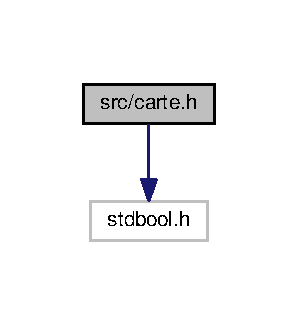
\includegraphics[width=143pt]{carte_8h__incl}
\end{center}
\end{figure}
Ce graphe montre quels fichiers incluent directement ou indirectement ce fichier \+:
\nopagebreak
\begin{figure}[H]
\begin{center}
\leavevmode
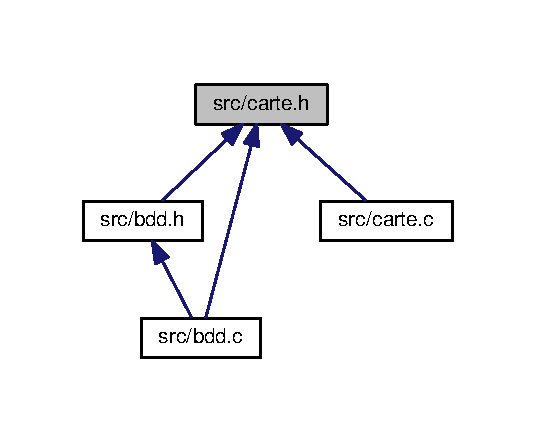
\includegraphics[width=257pt]{carte_8h__dep__incl}
\end{center}
\end{figure}
\subsection*{Structures de données}
\begin{DoxyCompactItemize}
\item 
struct \hyperlink{structcarte}{carte}
\item 
struct \hyperlink{structcarte__prop}{carte\+\_\+prop}
\end{DoxyCompactItemize}
\subsection*{Énumérations}
\begin{DoxyCompactItemize}
\item 
enum \hyperlink{carte_8h_a2b6a5add5e3db9028dff54f9c1acdde7}{carte\+\_\+enseigne} \{ \\*
{\bfseries ce\+Null} = 0, 
{\bfseries ce\+Pique}, 
{\bfseries ce\+Carreau}, 
{\bfseries ce\+Coeur}, 
\\*
{\bfseries ce\+Trefle}
 \}
\item 
enum \hyperlink{carte_8h_a323916cdb68cd0d5d8a1660ffb45ea4e}{carte\+\_\+valeur} \{ \\*
{\bfseries cv\+Null} = 0, 
{\bfseries cv\+As}, 
{\bfseries cv2}, 
{\bfseries cv3}, 
\\*
{\bfseries cv4}, 
{\bfseries cv5}, 
{\bfseries cv6}, 
{\bfseries cv7}, 
\\*
{\bfseries cv8}, 
{\bfseries cv9}, 
{\bfseries cv10}, 
{\bfseries cv\+Valet}, 
\\*
{\bfseries cv\+Dame}, 
{\bfseries cv\+Roi}
 \}
\item 
enum \hyperlink{carte_8h_a71a2818c25230a5e1a239f28c1e6deba}{carte\+\_\+prop\+\_\+type} \{ {\bfseries cpt\+Enseigne}, 
{\bfseries cpt\+Valeur}, 
{\bfseries cpt\+Peut\+Battre}
 \}
\end{DoxyCompactItemize}
\subsection*{Fonctions}
\begin{DoxyCompactItemize}
\item 
\hyperlink{structcarte__prop}{carte\+\_\+prop} $\ast$ \hyperlink{carte_8h_a49c3910a75cd95f3f2868811d6d10500}{air\+\_\+carte\+\_\+prop\+\_\+find\+\_\+type} (\hyperlink{structcarte__prop}{carte\+\_\+prop} $\ast$ptr, enum \hyperlink{carte_8h_a71a2818c25230a5e1a239f28c1e6deba}{carte\+\_\+prop\+\_\+type} type)
\begin{DoxyCompactList}\small\item\em Recherche la première propriété de type {\ttfamily type} dans la chaîne des propriétés d\textquotesingle{}une carte donnée. \end{DoxyCompactList}\item 
\hyperlink{structcarte__prop}{carte\+\_\+prop} $\ast$ \hyperlink{carte_8h_a3de298787ae5ff81eaf9b16caa6e2578}{air\+\_\+carte\+\_\+prop\+\_\+creer} ()
\begin{DoxyCompactList}\small\item\em Alloue la mémoire pour une \hyperlink{structcarte__prop}{carte\+\_\+prop} et l\textquotesingle{}initialise. \end{DoxyCompactList}\item 
int \hyperlink{carte_8h_ab931f47e29ed5f74a4b24f35503af391}{air\+\_\+carte\+\_\+prop\+\_\+ajouter} (\hyperlink{structcarte}{carte} $\ast$c, \hyperlink{structcarte__prop}{carte\+\_\+prop} $\ast$p)
\begin{DoxyCompactList}\small\item\em Ajoute une propriété à la carte. \end{DoxyCompactList}\item 
int \hyperlink{carte_8h_a1841a8f25ee0e8f4ee53f84b383772e4}{air\+\_\+carte\+\_\+prop\+\_\+init} (\hyperlink{structcarte__prop}{carte\+\_\+prop} $\ast$p)
\begin{DoxyCompactList}\small\item\em Initialise une \hyperlink{structcarte__prop}{carte\+\_\+prop}. \end{DoxyCompactList}\item 
\hyperlink{structcarte}{carte} $\ast$ \hyperlink{carte_8h_a3f348e02674aa3eefa118a2d1be7b77c}{air\+\_\+carte\+\_\+creer} ()
\begin{DoxyCompactList}\small\item\em Alloue dynamiquement une carte et l\textquotesingle{}initialise. \end{DoxyCompactList}\item 
void \hyperlink{carte_8h_a45274a3996ff9bed9e3d6e978655a1d4}{air\+\_\+carte\+\_\+free} (\hyperlink{structcarte}{carte} $\ast$c)
\begin{DoxyCompactList}\small\item\em Libère de la mémoire une carte. \end{DoxyCompactList}\item 
int \hyperlink{carte_8h_aca47330fc7b74166365ab3aea4d303a1}{air\+\_\+carte\+\_\+init} (\hyperlink{structcarte}{carte} $\ast$c)
\begin{DoxyCompactList}\small\item\em Initialise la structure. \end{DoxyCompactList}\item 
enum \hyperlink{carte_8h_a323916cdb68cd0d5d8a1660ffb45ea4e}{carte\+\_\+valeur} \hyperlink{carte_8h_ab411344f241870ba183d6c5db6c4898b}{air\+\_\+carte\+\_\+valeur\+\_\+get} (\hyperlink{structcarte}{carte} $\ast$c)
\begin{DoxyCompactList}\small\item\em Retourne la valeur d\textquotesingle{}une carte. \end{DoxyCompactList}\item 
int \hyperlink{carte_8h_addfb4cc8cdc67446e1fb2434bdbec2d0}{air\+\_\+carte\+\_\+valeur\+\_\+set} (\hyperlink{structcarte}{carte} $\ast$c, enum \hyperlink{carte_8h_a323916cdb68cd0d5d8a1660ffb45ea4e}{carte\+\_\+valeur} valeur)
\begin{DoxyCompactList}\small\item\em Affecte la valeur {\ttfamily valeur} à la carte. \end{DoxyCompactList}\item 
enum \hyperlink{carte_8h_a2b6a5add5e3db9028dff54f9c1acdde7}{carte\+\_\+enseigne} \hyperlink{carte_8h_a7dad267d5ce0603d60ddd72230aadc46}{air\+\_\+carte\+\_\+enseigne\+\_\+get} (\hyperlink{structcarte}{carte} $\ast$c)
\begin{DoxyCompactList}\small\item\em Retourne l\textquotesingle{}enseigne d\textquotesingle{}une carte. \end{DoxyCompactList}\item 
int \hyperlink{carte_8h_ad4dda778eb53e034326b558828cf2a40}{air\+\_\+carte\+\_\+enseigne\+\_\+set} (\hyperlink{structcarte}{carte} $\ast$c, enum \hyperlink{carte_8h_a2b6a5add5e3db9028dff54f9c1acdde7}{carte\+\_\+enseigne} enseigne)
\begin{DoxyCompactList}\small\item\em Affecte l\textquotesingle{}enseigne {\ttfamily enseigne} à la carte. \end{DoxyCompactList}\item 
bool \hyperlink{carte_8h_ad7eae524fba5e88efa3d7862655dd8df}{air\+\_\+carte\+\_\+peut\+\_\+battre} (\hyperlink{structcarte}{carte} $\ast$c, \hyperlink{structcarte}{carte} $\ast$peut\+\_\+battre)
\begin{DoxyCompactList}\small\item\em Vérifie si une carte peut en battre une autre. \end{DoxyCompactList}\item 
int \hyperlink{carte_8h_a63216eb2cdd6219203225de97f47c251}{air\+\_\+carte\+\_\+bat\+\_\+add} (\hyperlink{structcarte}{carte} $\ast$c, \hyperlink{structcarte}{carte} $\ast$peut\+\_\+battre)
\begin{DoxyCompactList}\small\item\em Affecte à une carte une référence vers une autre carte. \end{DoxyCompactList}\item 
void \hyperlink{carte_8h_ac6c44bf3c40f97468e22dcebfb622a6b}{air\+\_\+carte\+\_\+printf} (\hyperlink{structcarte}{carte} $\ast$c)
\begin{DoxyCompactList}\small\item\em Affiche les propriétés d\textquotesingle{}une carte sur la sortie standard. \end{DoxyCompactList}\item 
void \hyperlink{carte_8h_ae6ffa5f0d892f4d19b569f4ebc46564e}{air\+\_\+carte\+\_\+affiche\+\_\+valeur} (enum \hyperlink{carte_8h_a323916cdb68cd0d5d8a1660ffb45ea4e}{carte\+\_\+valeur} valeur)
\begin{DoxyCompactList}\small\item\em Affiche la valeur passée en paramètre dans la sortie standard. \end{DoxyCompactList}\item 
void \hyperlink{carte_8h_aa5514ebef2fa8a1d26628f153c3768e8}{air\+\_\+carte\+\_\+affiche\+\_\+enseigne} (enum \hyperlink{carte_8h_a2b6a5add5e3db9028dff54f9c1acdde7}{carte\+\_\+enseigne} enseigne)
\begin{DoxyCompactList}\small\item\em Affiche l\textquotesingle{}enseigne passée en paramètre dans la sortie standard. \end{DoxyCompactList}\end{DoxyCompactItemize}


\subsection{Description détaillée}
Définition des fonctions et types de cartes. 

\begin{DoxyAuthor}{Auteur}
Loïc Payol \href{mailto:loicpayol@gmail.com}{\tt loicpayol@gmail.\+com} 
\end{DoxyAuthor}


\subsection{Documentation du type de l\textquotesingle{}énumération}
\index{carte.\+h@{carte.\+h}!carte\+\_\+enseigne@{carte\+\_\+enseigne}}
\index{carte\+\_\+enseigne@{carte\+\_\+enseigne}!carte.\+h@{carte.\+h}}
\subsubsection[{\texorpdfstring{carte\+\_\+enseigne}{carte_enseigne}}]{\setlength{\rightskip}{0pt plus 5cm}enum {\bf carte\+\_\+enseigne}}\hypertarget{carte_8h_a2b6a5add5e3db9028dff54f9c1acdde7}{}\label{carte_8h_a2b6a5add5e3db9028dff54f9c1acdde7}
Définit les enseigne d\textquotesingle{}une carte \index{carte.\+h@{carte.\+h}!carte\+\_\+prop\+\_\+type@{carte\+\_\+prop\+\_\+type}}
\index{carte\+\_\+prop\+\_\+type@{carte\+\_\+prop\+\_\+type}!carte.\+h@{carte.\+h}}
\subsubsection[{\texorpdfstring{carte\+\_\+prop\+\_\+type}{carte_prop_type}}]{\setlength{\rightskip}{0pt plus 5cm}enum {\bf carte\+\_\+prop\+\_\+type}}\hypertarget{carte_8h_a71a2818c25230a5e1a239f28c1e6deba}{}\label{carte_8h_a71a2818c25230a5e1a239f28c1e6deba}
Enumération pour le champ discriminant de l\textquotesingle{}union \index{carte.\+h@{carte.\+h}!carte\+\_\+valeur@{carte\+\_\+valeur}}
\index{carte\+\_\+valeur@{carte\+\_\+valeur}!carte.\+h@{carte.\+h}}
\subsubsection[{\texorpdfstring{carte\+\_\+valeur}{carte_valeur}}]{\setlength{\rightskip}{0pt plus 5cm}enum {\bf carte\+\_\+valeur}}\hypertarget{carte_8h_a323916cdb68cd0d5d8a1660ffb45ea4e}{}\label{carte_8h_a323916cdb68cd0d5d8a1660ffb45ea4e}
Définit les valeurs d\textquotesingle{}une carte 

\subsection{Documentation des fonctions}
\index{carte.\+h@{carte.\+h}!air\+\_\+carte\+\_\+affiche\+\_\+enseigne@{air\+\_\+carte\+\_\+affiche\+\_\+enseigne}}
\index{air\+\_\+carte\+\_\+affiche\+\_\+enseigne@{air\+\_\+carte\+\_\+affiche\+\_\+enseigne}!carte.\+h@{carte.\+h}}
\subsubsection[{\texorpdfstring{air\+\_\+carte\+\_\+affiche\+\_\+enseigne(enum carte\+\_\+enseigne enseigne)}{air_carte_affiche_enseigne(enum carte_enseigne enseigne)}}]{\setlength{\rightskip}{0pt plus 5cm}void air\+\_\+carte\+\_\+affiche\+\_\+enseigne (
\begin{DoxyParamCaption}
\item[{enum {\bf carte\+\_\+enseigne}}]{enseigne}
\end{DoxyParamCaption}
)}\hypertarget{carte_8h_aa5514ebef2fa8a1d26628f153c3768e8}{}\label{carte_8h_aa5514ebef2fa8a1d26628f153c3768e8}


Affiche l\textquotesingle{}enseigne passée en paramètre dans la sortie standard. 


\begin{DoxyParams}{Paramètres}
{\em valeur} & L\textquotesingle{}enseigne à afficher \\
\hline
\end{DoxyParams}
\index{carte.\+h@{carte.\+h}!air\+\_\+carte\+\_\+affiche\+\_\+valeur@{air\+\_\+carte\+\_\+affiche\+\_\+valeur}}
\index{air\+\_\+carte\+\_\+affiche\+\_\+valeur@{air\+\_\+carte\+\_\+affiche\+\_\+valeur}!carte.\+h@{carte.\+h}}
\subsubsection[{\texorpdfstring{air\+\_\+carte\+\_\+affiche\+\_\+valeur(enum carte\+\_\+valeur valeur)}{air_carte_affiche_valeur(enum carte_valeur valeur)}}]{\setlength{\rightskip}{0pt plus 5cm}void air\+\_\+carte\+\_\+affiche\+\_\+valeur (
\begin{DoxyParamCaption}
\item[{enum {\bf carte\+\_\+valeur}}]{valeur}
\end{DoxyParamCaption}
)}\hypertarget{carte_8h_ae6ffa5f0d892f4d19b569f4ebc46564e}{}\label{carte_8h_ae6ffa5f0d892f4d19b569f4ebc46564e}


Affiche la valeur passée en paramètre dans la sortie standard. 


\begin{DoxyParams}{Paramètres}
{\em valeur} & La valeur à afficher \\
\hline
\end{DoxyParams}
\index{carte.\+h@{carte.\+h}!air\+\_\+carte\+\_\+bat\+\_\+add@{air\+\_\+carte\+\_\+bat\+\_\+add}}
\index{air\+\_\+carte\+\_\+bat\+\_\+add@{air\+\_\+carte\+\_\+bat\+\_\+add}!carte.\+h@{carte.\+h}}
\subsubsection[{\texorpdfstring{air\+\_\+carte\+\_\+bat\+\_\+add(carte $\ast$c, carte $\ast$peut\+\_\+battre)}{air_carte_bat_add(carte *c, carte *peut_battre)}}]{\setlength{\rightskip}{0pt plus 5cm}int air\+\_\+carte\+\_\+bat\+\_\+add (
\begin{DoxyParamCaption}
\item[{{\bf carte} $\ast$}]{c, }
\item[{{\bf carte} $\ast$}]{peut\+\_\+battre}
\end{DoxyParamCaption}
)}\hypertarget{carte_8h_a63216eb2cdd6219203225de97f47c251}{}\label{carte_8h_a63216eb2cdd6219203225de97f47c251}


Affecte à une carte une référence vers une autre carte. 


\begin{DoxyParams}{Paramètres}
{\em c} & L\textquotesingle{}instance de la structure à modifier \\
\hline
{\em peut\+\_\+battre} & La carte battue \\
\hline
\end{DoxyParams}
\begin{DoxyReturn}{Renvoie}
0 lorsqu\textquotesingle{}aucune erreur n\textquotesingle{}a eu lieu, -\/1 quand une erreur a eu lieu (peut\+\_\+battre == N\+U\+LL ou à c) 
\end{DoxyReturn}
\index{carte.\+h@{carte.\+h}!air\+\_\+carte\+\_\+creer@{air\+\_\+carte\+\_\+creer}}
\index{air\+\_\+carte\+\_\+creer@{air\+\_\+carte\+\_\+creer}!carte.\+h@{carte.\+h}}
\subsubsection[{\texorpdfstring{air\+\_\+carte\+\_\+creer()}{air_carte_creer()}}]{\setlength{\rightskip}{0pt plus 5cm}{\bf carte}$\ast$ air\+\_\+carte\+\_\+creer (
\begin{DoxyParamCaption}
{}
\end{DoxyParamCaption}
)}\hypertarget{carte_8h_a3f348e02674aa3eefa118a2d1be7b77c}{}\label{carte_8h_a3f348e02674aa3eefa118a2d1be7b77c}


Alloue dynamiquement une carte et l\textquotesingle{}initialise. 

\begin{DoxyReturn}{Renvoie}
N\+U\+LL en cas d\textquotesingle{}erreur (voir errno), sinon la carte nouvellement créée 
\end{DoxyReturn}
\index{carte.\+h@{carte.\+h}!air\+\_\+carte\+\_\+enseigne\+\_\+get@{air\+\_\+carte\+\_\+enseigne\+\_\+get}}
\index{air\+\_\+carte\+\_\+enseigne\+\_\+get@{air\+\_\+carte\+\_\+enseigne\+\_\+get}!carte.\+h@{carte.\+h}}
\subsubsection[{\texorpdfstring{air\+\_\+carte\+\_\+enseigne\+\_\+get(carte $\ast$c)}{air_carte_enseigne_get(carte *c)}}]{\setlength{\rightskip}{0pt plus 5cm}enum {\bf carte\+\_\+enseigne} air\+\_\+carte\+\_\+enseigne\+\_\+get (
\begin{DoxyParamCaption}
\item[{{\bf carte} $\ast$}]{c}
\end{DoxyParamCaption}
)}\hypertarget{carte_8h_a7dad267d5ce0603d60ddd72230aadc46}{}\label{carte_8h_a7dad267d5ce0603d60ddd72230aadc46}


Retourne l\textquotesingle{}enseigne d\textquotesingle{}une carte. 


\begin{DoxyParams}{Paramètres}
{\em c} & La carte \\
\hline
\end{DoxyParams}
\begin{DoxyReturn}{Renvoie}
L\textquotesingle{}enseigne de la carte 
\end{DoxyReturn}
\index{carte.\+h@{carte.\+h}!air\+\_\+carte\+\_\+enseigne\+\_\+set@{air\+\_\+carte\+\_\+enseigne\+\_\+set}}
\index{air\+\_\+carte\+\_\+enseigne\+\_\+set@{air\+\_\+carte\+\_\+enseigne\+\_\+set}!carte.\+h@{carte.\+h}}
\subsubsection[{\texorpdfstring{air\+\_\+carte\+\_\+enseigne\+\_\+set(carte $\ast$c, enum carte\+\_\+enseigne enseigne)}{air_carte_enseigne_set(carte *c, enum carte_enseigne enseigne)}}]{\setlength{\rightskip}{0pt plus 5cm}int air\+\_\+carte\+\_\+enseigne\+\_\+set (
\begin{DoxyParamCaption}
\item[{{\bf carte} $\ast$}]{c, }
\item[{enum {\bf carte\+\_\+enseigne}}]{enseigne}
\end{DoxyParamCaption}
)}\hypertarget{carte_8h_ad4dda778eb53e034326b558828cf2a40}{}\label{carte_8h_ad4dda778eb53e034326b558828cf2a40}


Affecte l\textquotesingle{}enseigne {\ttfamily enseigne} à la carte. 


\begin{DoxyParams}{Paramètres}
{\em c} & L\textquotesingle{}instance de la structure à modifier \\
\hline
{\em enseigne} & L\textquotesingle{}enseigne à affecter \\
\hline
\end{DoxyParams}
\begin{DoxyReturn}{Renvoie}
0 lorsqu\textquotesingle{}aucune erreur n\textquotesingle{}a eu lieu 
\end{DoxyReturn}
\index{carte.\+h@{carte.\+h}!air\+\_\+carte\+\_\+free@{air\+\_\+carte\+\_\+free}}
\index{air\+\_\+carte\+\_\+free@{air\+\_\+carte\+\_\+free}!carte.\+h@{carte.\+h}}
\subsubsection[{\texorpdfstring{air\+\_\+carte\+\_\+free(carte $\ast$c)}{air_carte_free(carte *c)}}]{\setlength{\rightskip}{0pt plus 5cm}void air\+\_\+carte\+\_\+free (
\begin{DoxyParamCaption}
\item[{{\bf carte} $\ast$}]{c}
\end{DoxyParamCaption}
)}\hypertarget{carte_8h_a45274a3996ff9bed9e3d6e978655a1d4}{}\label{carte_8h_a45274a3996ff9bed9e3d6e978655a1d4}


Libère de la mémoire une carte. 


\begin{DoxyParams}{Paramètres}
{\em c} & La carte à libérer de la mémoire \\
\hline
\end{DoxyParams}
\index{carte.\+h@{carte.\+h}!air\+\_\+carte\+\_\+init@{air\+\_\+carte\+\_\+init}}
\index{air\+\_\+carte\+\_\+init@{air\+\_\+carte\+\_\+init}!carte.\+h@{carte.\+h}}
\subsubsection[{\texorpdfstring{air\+\_\+carte\+\_\+init(carte $\ast$c)}{air_carte_init(carte *c)}}]{\setlength{\rightskip}{0pt plus 5cm}int air\+\_\+carte\+\_\+init (
\begin{DoxyParamCaption}
\item[{{\bf carte} $\ast$}]{c}
\end{DoxyParamCaption}
)}\hypertarget{carte_8h_aca47330fc7b74166365ab3aea4d303a1}{}\label{carte_8h_aca47330fc7b74166365ab3aea4d303a1}


Initialise la structure. 


\begin{DoxyParams}{Paramètres}
{\em c} & L\textquotesingle{}instance de la structure à initialiser \\
\hline
\end{DoxyParams}
\begin{DoxyReturn}{Renvoie}
0 lorsqu\textquotesingle{}aucune erreur n\textquotesingle{}a eu lieu 
\end{DoxyReturn}
\index{carte.\+h@{carte.\+h}!air\+\_\+carte\+\_\+peut\+\_\+battre@{air\+\_\+carte\+\_\+peut\+\_\+battre}}
\index{air\+\_\+carte\+\_\+peut\+\_\+battre@{air\+\_\+carte\+\_\+peut\+\_\+battre}!carte.\+h@{carte.\+h}}
\subsubsection[{\texorpdfstring{air\+\_\+carte\+\_\+peut\+\_\+battre(carte $\ast$c, carte $\ast$peut\+\_\+battre)}{air_carte_peut_battre(carte *c, carte *peut_battre)}}]{\setlength{\rightskip}{0pt plus 5cm}bool air\+\_\+carte\+\_\+peut\+\_\+battre (
\begin{DoxyParamCaption}
\item[{{\bf carte} $\ast$}]{c, }
\item[{{\bf carte} $\ast$}]{peut\+\_\+battre}
\end{DoxyParamCaption}
)}\hypertarget{carte_8h_ad7eae524fba5e88efa3d7862655dd8df}{}\label{carte_8h_ad7eae524fba5e88efa3d7862655dd8df}


Vérifie si une carte peut en battre une autre. 


\begin{DoxyParams}{Paramètres}
{\em c} & La carte \char`\"{}attaquante\char`\"{} \\
\hline
{\em peut\+\_\+battre} & La carte \char`\"{}attaquée\char`\"{} \\
\hline
\end{DoxyParams}
\begin{DoxyReturn}{Renvoie}
true si la carte attaquante peut la battre, false sinon 
\end{DoxyReturn}
\index{carte.\+h@{carte.\+h}!air\+\_\+carte\+\_\+printf@{air\+\_\+carte\+\_\+printf}}
\index{air\+\_\+carte\+\_\+printf@{air\+\_\+carte\+\_\+printf}!carte.\+h@{carte.\+h}}
\subsubsection[{\texorpdfstring{air\+\_\+carte\+\_\+printf(carte $\ast$c)}{air_carte_printf(carte *c)}}]{\setlength{\rightskip}{0pt plus 5cm}void air\+\_\+carte\+\_\+printf (
\begin{DoxyParamCaption}
\item[{{\bf carte} $\ast$}]{c}
\end{DoxyParamCaption}
)}\hypertarget{carte_8h_ac6c44bf3c40f97468e22dcebfb622a6b}{}\label{carte_8h_ac6c44bf3c40f97468e22dcebfb622a6b}


Affiche les propriétés d\textquotesingle{}une carte sur la sortie standard. 


\begin{DoxyParams}{Paramètres}
{\em c} & La carte à afficher \\
\hline
\end{DoxyParams}
\index{carte.\+h@{carte.\+h}!air\+\_\+carte\+\_\+prop\+\_\+ajouter@{air\+\_\+carte\+\_\+prop\+\_\+ajouter}}
\index{air\+\_\+carte\+\_\+prop\+\_\+ajouter@{air\+\_\+carte\+\_\+prop\+\_\+ajouter}!carte.\+h@{carte.\+h}}
\subsubsection[{\texorpdfstring{air\+\_\+carte\+\_\+prop\+\_\+ajouter(carte $\ast$c, carte\+\_\+prop $\ast$p)}{air_carte_prop_ajouter(carte *c, carte_prop *p)}}]{\setlength{\rightskip}{0pt plus 5cm}int air\+\_\+carte\+\_\+prop\+\_\+ajouter (
\begin{DoxyParamCaption}
\item[{{\bf carte} $\ast$}]{c, }
\item[{{\bf carte\+\_\+prop} $\ast$}]{p}
\end{DoxyParamCaption}
)}\hypertarget{carte_8h_ab931f47e29ed5f74a4b24f35503af391}{}\label{carte_8h_ab931f47e29ed5f74a4b24f35503af391}


Ajoute une propriété à la carte. 


\begin{DoxyParams}{Paramètres}
{\em c} & La carte à modifier \\
\hline
{\em p} & La propriété à ajouter \\
\hline
\end{DoxyParams}
\begin{DoxyReturn}{Renvoie}
0 lorsqu\textquotesingle{}aucune erreur n\textquotesingle{}a eu lieu 
\end{DoxyReturn}
\index{carte.\+h@{carte.\+h}!air\+\_\+carte\+\_\+prop\+\_\+creer@{air\+\_\+carte\+\_\+prop\+\_\+creer}}
\index{air\+\_\+carte\+\_\+prop\+\_\+creer@{air\+\_\+carte\+\_\+prop\+\_\+creer}!carte.\+h@{carte.\+h}}
\subsubsection[{\texorpdfstring{air\+\_\+carte\+\_\+prop\+\_\+creer()}{air_carte_prop_creer()}}]{\setlength{\rightskip}{0pt plus 5cm}{\bf carte\+\_\+prop}$\ast$ air\+\_\+carte\+\_\+prop\+\_\+creer (
\begin{DoxyParamCaption}
{}
\end{DoxyParamCaption}
)}\hypertarget{carte_8h_a3de298787ae5ff81eaf9b16caa6e2578}{}\label{carte_8h_a3de298787ae5ff81eaf9b16caa6e2578}


Alloue la mémoire pour une \hyperlink{structcarte__prop}{carte\+\_\+prop} et l\textquotesingle{}initialise. 

\begin{DoxyReturn}{Renvoie}
N\+U\+LL en cas d\textquotesingle{}erreur (voir errno), sinon la prorpiété nouvellement créée 
\end{DoxyReturn}
\index{carte.\+h@{carte.\+h}!air\+\_\+carte\+\_\+prop\+\_\+find\+\_\+type@{air\+\_\+carte\+\_\+prop\+\_\+find\+\_\+type}}
\index{air\+\_\+carte\+\_\+prop\+\_\+find\+\_\+type@{air\+\_\+carte\+\_\+prop\+\_\+find\+\_\+type}!carte.\+h@{carte.\+h}}
\subsubsection[{\texorpdfstring{air\+\_\+carte\+\_\+prop\+\_\+find\+\_\+type(carte\+\_\+prop $\ast$ptr, enum carte\+\_\+prop\+\_\+type type)}{air_carte_prop_find_type(carte_prop *ptr, enum carte_prop_type type)}}]{\setlength{\rightskip}{0pt plus 5cm}{\bf carte\+\_\+prop}$\ast$ air\+\_\+carte\+\_\+prop\+\_\+find\+\_\+type (
\begin{DoxyParamCaption}
\item[{{\bf carte\+\_\+prop} $\ast$}]{ptr, }
\item[{enum {\bf carte\+\_\+prop\+\_\+type}}]{type}
\end{DoxyParamCaption}
)}\hypertarget{carte_8h_a49c3910a75cd95f3f2868811d6d10500}{}\label{carte_8h_a49c3910a75cd95f3f2868811d6d10500}


Recherche la première propriété de type {\ttfamily type} dans la chaîne des propriétés d\textquotesingle{}une carte donnée. 


\begin{DoxyParams}{Paramètres}
{\em ptr} & La propriété à partir de laquelle effectuer la recherche \\
\hline
{\em type} & Le type à rechercher \\
\hline
\end{DoxyParams}
\index{carte.\+h@{carte.\+h}!air\+\_\+carte\+\_\+prop\+\_\+init@{air\+\_\+carte\+\_\+prop\+\_\+init}}
\index{air\+\_\+carte\+\_\+prop\+\_\+init@{air\+\_\+carte\+\_\+prop\+\_\+init}!carte.\+h@{carte.\+h}}
\subsubsection[{\texorpdfstring{air\+\_\+carte\+\_\+prop\+\_\+init(carte\+\_\+prop $\ast$p)}{air_carte_prop_init(carte_prop *p)}}]{\setlength{\rightskip}{0pt plus 5cm}int air\+\_\+carte\+\_\+prop\+\_\+init (
\begin{DoxyParamCaption}
\item[{{\bf carte\+\_\+prop} $\ast$}]{p}
\end{DoxyParamCaption}
)}\hypertarget{carte_8h_a1841a8f25ee0e8f4ee53f84b383772e4}{}\label{carte_8h_a1841a8f25ee0e8f4ee53f84b383772e4}


Initialise une \hyperlink{structcarte__prop}{carte\+\_\+prop}. 


\begin{DoxyParams}{Paramètres}
{\em p} & La propriété à initialiser \\
\hline
\end{DoxyParams}
\begin{DoxyReturn}{Renvoie}
0 lorsqu\textquotesingle{}aucune erreur n\textquotesingle{}a eu lieu 
\end{DoxyReturn}
\index{carte.\+h@{carte.\+h}!air\+\_\+carte\+\_\+valeur\+\_\+get@{air\+\_\+carte\+\_\+valeur\+\_\+get}}
\index{air\+\_\+carte\+\_\+valeur\+\_\+get@{air\+\_\+carte\+\_\+valeur\+\_\+get}!carte.\+h@{carte.\+h}}
\subsubsection[{\texorpdfstring{air\+\_\+carte\+\_\+valeur\+\_\+get(carte $\ast$c)}{air_carte_valeur_get(carte *c)}}]{\setlength{\rightskip}{0pt plus 5cm}enum {\bf carte\+\_\+valeur} air\+\_\+carte\+\_\+valeur\+\_\+get (
\begin{DoxyParamCaption}
\item[{{\bf carte} $\ast$}]{c}
\end{DoxyParamCaption}
)}\hypertarget{carte_8h_ab411344f241870ba183d6c5db6c4898b}{}\label{carte_8h_ab411344f241870ba183d6c5db6c4898b}


Retourne la valeur d\textquotesingle{}une carte. 


\begin{DoxyParams}{Paramètres}
{\em c} & La carte \\
\hline
\end{DoxyParams}
\begin{DoxyReturn}{Renvoie}
La valeur de la carte 
\end{DoxyReturn}
\index{carte.\+h@{carte.\+h}!air\+\_\+carte\+\_\+valeur\+\_\+set@{air\+\_\+carte\+\_\+valeur\+\_\+set}}
\index{air\+\_\+carte\+\_\+valeur\+\_\+set@{air\+\_\+carte\+\_\+valeur\+\_\+set}!carte.\+h@{carte.\+h}}
\subsubsection[{\texorpdfstring{air\+\_\+carte\+\_\+valeur\+\_\+set(carte $\ast$c, enum carte\+\_\+valeur valeur)}{air_carte_valeur_set(carte *c, enum carte_valeur valeur)}}]{\setlength{\rightskip}{0pt plus 5cm}int air\+\_\+carte\+\_\+valeur\+\_\+set (
\begin{DoxyParamCaption}
\item[{{\bf carte} $\ast$}]{c, }
\item[{enum {\bf carte\+\_\+valeur}}]{valeur}
\end{DoxyParamCaption}
)}\hypertarget{carte_8h_addfb4cc8cdc67446e1fb2434bdbec2d0}{}\label{carte_8h_addfb4cc8cdc67446e1fb2434bdbec2d0}


Affecte la valeur {\ttfamily valeur} à la carte. 


\begin{DoxyParams}{Paramètres}
{\em c} & L\textquotesingle{}instance de la structure à modifier \\
\hline
{\em valeur} & La valeur à affecter \\
\hline
\end{DoxyParams}
\begin{DoxyReturn}{Renvoie}
0 lorsqu\textquotesingle{}aucune erreur n\textquotesingle{}a eu lieu 
\end{DoxyReturn}

%--- End generated contents ---

% Index
\backmatter
\newpage
\phantomsection
\clearemptydoublepage
\addcontentsline{toc}{chapter}{Index}
\printindex

\end{document}
